\chapter{Experimentos \& Análises}
\label{cap6}



A partir dos dados coletados, foi realizada uma análise dos dados seguindo os critérios levantados durante a proposta do atual trabalho.
%
Tal análise visa compreender o consumo dos recursos empregados pelas arquiteturas com base em suas características específicas.



Cada caso de análise é dividido em experimentos, no qual cada experimento tem o objetivo de analisar um conjunto de recursos dado algum cenário.
%
Faz sentido subdividir tais experimentos em grupos menores, para posterior comparação.



%ccm todo gráfico precisa responder a alguma pergunta.
% 1- Formular a pergunta com base no que definiu no Cap.4
% 2- quem está envolvido, quais são os parâmetros, quais são constantes
% 3- Descrever o perfil/modus operandi do experimento
% 4- Mostrar a figura
% 5- Analisar os resultados com base na expectativa no Cap.4 (foi similar, diferente, por quê?)
% 6 - Precisa manter em mente que as figuras devem manter uma escala para poder comparar entre diferentes arquiteturas


\section{Experimentos}
\label{sec:experimentos}

Cada experimento utiliza as arquiteturas de microsserviços para jogos \ac{mmorpg} Rudy, Salz e Willson.
%
Cada arquitetura é executada no mesmo ambiente, devidamente isolado, em momentos diferentes.
%
Para cada arquitetura, foram realizadas três execuções com os mesmos parâmetros, a fim de assegurar que um padrão de comportamento existe.
%
Cada  experimento é executado seguindo o protocolo:


\begin{enumerate}
 \item Início dos serviços do banco de dados.
 \item Início dos serviços de jogo.
 \item Início dos clientes.
 \item Clientes são adicionados de 1 em 1, a cada 30 segundos, até atingir a quantidade de 100 clientes simultâneos.
 \item Após a finalização do experimento os serviços em todos os ambientes são removidos, mantendo somente os dados capturados.
\end{enumerate}


A partir de tais execuções os dados são capturados, processados e analisados.
%
Durante as execuções, os dados sobre a latência entre a rede do serviço e cliente mostrou-se estável, variando entre 5ms e 15ms, dessa forma foram ignorados como um experimento a parte, porém tal dado serve para validar a estabilidade da rede.

\subsection{Tempo de Resposta}

Este experimento visa analisar o tempo de resposta em relação ao número de jogadores simultâneos.
%
Espera-se que o seu crescimento seja de tendência linear junto ao crescimento de jogadores concorrentes.
%
Neste contexto existem as seguintes variáveis:

\begin{itemize}
    \item Jogadores simultâneos: Variável capturada a partir do microsserviço de jogo; e
    \item Tempo de Resposta: Variável capturada a partir dos clientes.
\end{itemize}

Tal experimento permitirá analisar a qualidade das arquiteturas de microsserviços, do ponto de vista do cliente em relação ao tempo de resposta.
%
As características observadas nestas análises servem também como critério de desempate nas análises de experimentos seguintes.

Nota-se que o número de jogadores simultâneos e o tempo de resposta são indexados pelo tempo na qual tais dados foram capturados.
%
Nesse sentido, pode-se relacionar o tempo de resposta de todos os clientes ao número de jogadores simultâneos.
%
Dado tal contexto, faz sentido realizar uma análise separando os ambientes baseando-se em algumas ações na qual operam sobre microsserviços e recursos diferentes.

Dentro deste contexto existem dois tipos de requisições: as que não pertencem a estrutura de repetição infinita do autômato do cliente e as requisições que pertencem a estrutura de repetição infinita do autômato do cliente.
%
As requisições que não pertencem a estrutura de repetição infinita são:

\begin{itemize}
    \item Criar conta;
    \item Criar personagem;
    \item Iniciar sessão; e
    \item Instanciar personagem.
\end{itemize}

As requisições que pertencem a estrutura de repetição infinita são:

\begin{itemize}
    \item Movimentar personagem;
    \item Enviar mensagem; e
    \item Receber mensagem.
\end{itemize}


\subsubsection{Criar conta}
\label{sec:op_create_account}

A operação de criar conta é efetuada sobre o protocolo \ac{tcp}/\ac{http}.
%
Nesta operação, o cliente envia um formulário em formato \ac{json} com informações básicas comuns em jogos \ac{mmorpg} para uma instância de conta.
%
Os dados são validados e inseridos no banco de dados, caso a validação esteja correta.

Uma característica importante para este experimento é a quantidade de requisições efetuadas, a qual é apresentada ao exibir a sua frequência no tempo de contato entre um usuário desta aplicação e o serviço.
%
A tendência é que um usuário realize uma única requisição durante todo o seu tempo de vida ao entrar em contato com algum jogo \ac{mmorpg}.

O microsserviço responsável por receber estas requisições não lida com concorrência conforme a demanda dos jogadores simultâneos, sendo assim o tempo de resposta não deve variar conforme o aumento do número de jogadores simultâneos.
%
A Figura~\ref{fig:create_account_operation_request_time} torna visível que o comportamento do tempo de resposta não depende do número de jogadores simultâneos.

\begin{figure}[htb!]
  \caption{Tempo de resposta para criar contas}
  \label{fig:create_account_operation_request_time}
  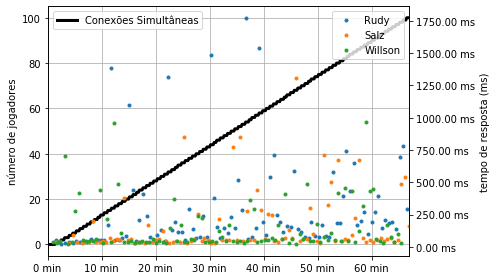
\includegraphics[width=0.8\textwidth]{figuras/analise/rt/create_account_operation_request_time.png}
  \centering

  Fonte: O próprio autor.
\end{figure}

Torna-se notório uma disparidade na Figura~\ref{fig:create_account_operation_request_time} entre os tempos de resposta coletados, conforme a arquitetura utilizada.
%
Esta disparidade exibe pontos discrepantes na execução da operação de criação de conta.

Dado o contexto, esta disparidade é resultado da concorrência no acesso ao banco por outras operações, as quais impactam diretamente a coleta do tempo de resposta desse experimento.
%
Nesse sentido, existe pela natureza da formação dos serviços, uma diferença no tempo de resposta perceptível aos clientes.

Para quantificar a Figura~\ref{fig:create_account_operation_request_time} faz sentido buscar os valores de média, variância, máximo e mínimo dos dados obtidos.
%
A Tabela~\ref{tab:create_account_operation_request_time} exibe estes valores estatísticos.

\begin{table}[htb!]
\centering
\begin{adjustbox}{max width=\textwidth}
\caption{Média, Variância, Máximo e Mínimo da operação Criar Conta}
\label{tab:create_account_operation_request_time}
\begin{tabular}{l|l|l|l|l}
\hline \hline
Arquitetura & Média     & Variância & Máximo    & Mínimo  \\ \hline \hline
Rudy        & 263,09 ms & 115701,29 & 1774,0 ms & 19,0 ms \\ \hline
Salz        & 152,53 ms & 50575,35  & 1304,0 ms & 28,0 ms \\ \hline
Willson     & 135,98 ms & 30573,78  & 968,0 ms  & 20,0 ms \\ \hline \hline
\end{tabular}

\end{adjustbox}
\end{table}

Como exibido na Tabela~\ref{tab:create_account_operation_request_time}, pode-se perceber que existe uma diferença abrupta na média de tempo de resposta da \ac{api} e sua respectiva variância.
%
Os valores de máximo e mínimo somente são exibidos como pontos de atenção, entretanto, como visível na Figura~\ref{fig:create_account_operation_request_time} são poucas requisições que não pertencem a tendência na região de maior densidade de requisições, justificando sua variância.

No contexto do atual trabalho, pode-se assumir a variância como disparidade entre os dados.
%
Quanto maior o valor, mais instável é o tempo de resposta de determinada operação ao ser requisitada ao serviço, entretanto, mesmo sendo instável tenderá a responder em uma média de tempo determinado.

A partir deste contexto, pode-se definir que a média de tempo de resposta do serviço, ao criar uma nova conta, segue a seguinte relação:

$$
  \overline{CriarConta_{w}} < \overline{CriarConta_{s}} < \overline{CriarConta_{r}}
$$

Deste modo, entende-se:

\begin{itemize}
 \item $\overline{CriarConta_{r}}$: Tempo de resposta médio da operação criar conta na arquitetura Rudy;
 \item $\overline{CriarConta_{s}}$: Tempo de resposta médio da operação criar conta na arquitetura Salz; e
 \item $\overline{CriarConta_{w}}$: Tempo de resposta médio da operação criar conta na arquitetura Willson.
\end{itemize}

Dessa forma, pode-se dizer que para a operação de criar conta, em média do ponto de vista de tempo de resposta, a arquitetura Willson é superior a arquitetura Salz e Rudy, respectivamente.
%
Também pode-se afirmar que a estabilidade desta operação, do ponto de vista de tempo de resposta, também segue a mesma sequência.
%ccm Indentificou melhor mas não justificou a origem dessa melhora

\subsubsection{Criar personagem}
\label{sec:op_create_char}

A operação de criar de personagem é efetuada sobre o protocolo \ac{tcp}/\ac{http}.
%
Nesta operação, o cliente envia um formulário em formato \ac{json} com informações básicas comuns em jogos \ac{mmorpg} para uma instância de personagem e dados de autenticação da conta.
%
Os dados são validados e inseridos no banco de dados, caso a validação esteja correta.

\begin{figure}[htb!]
  \caption{Tempo de resposta para criar personagens}
  \label{fig:create_character_operation_request}
  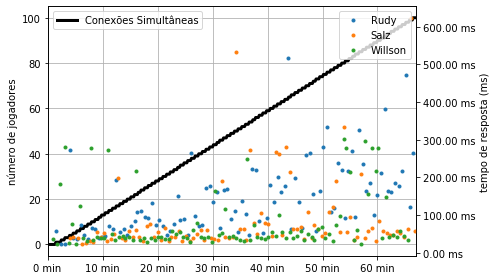
\includegraphics[width=0.8\textwidth]{figuras/analise/rt/create_character_operation_request.png}
  \centering

  Fonte: O próprio autor.
\end{figure}

Como pode-se perceber, através da Figura~\ref{fig:create_character_operation_request}, o comportamento do tempo de resposta da perspectiva do cliente é similar a operação criar conta (Subseção~\ref{sec:op_create_account}).
%
Sendo assim, faz sentido aplicar o mesmo método de análise para validar a existência de comportamentos similares, haja vista que a natureza desta operação é similar a criação de personagem.

Seguindo o método da média dos dados obtidos, pode-se obter os valores de média, variância, máximo e mínimo.
%
É possível visualizar estes valores na Tabela~\ref{tab:create_character_operation_request}.

\begin{table}[htb!]
\centering
\begin{adjustbox}{max width=\textwidth}
\caption{Média, Variância, Máximo e Mínimo da operação Criar Personagem}
\label{tab:create_character_operation_request}
\begin{tabular}{l|l|l|l|l}
\hline \hline
Arquitetura & Média     & Variância & Máximo    & Mínimo  \\ \hline \hline
Rudy        & 135,43 ms & 8782,99 & 517,0 ms & 23,0 ms \\ \hline
Salz        & 82,48 ms & 9106,62  & 624,0 ms & 24,0 ms \\ \hline
Willson     & 73,66 ms & 4886,60  & 301,0 ms  & 22,0 ms \\ \hline \hline
\end{tabular}

\end{adjustbox}

Fonte: O próprio autor.
\end{table}

A partir da Tabela~\ref{tab:create_character_operation_request}, pode-se observar que a média dos valores segue o comportamento encontrado na operação Criar Conta (Subseção~\ref{sec:op_create_account}). 
%
Entretanto, é notório a diferença com relação a estabilidade da operação de criação de personagem.

Para realizar esta operação, o serviço realiza diversas validações, geralmente efetuando a troca de mensagens entre os microsserviços de autenticação e validações de campos.
%
Tal situação, diferente da operação Criar Conta (Subseção~\ref{sec:op_create_account}), realiza poucas validações lógicas de regra de negócio, aplicando-as diretamente ao banco de dados PostgreSQL.

A partir desta característica, pode-se analisar a diferença na estabilidade entre as arquiteturas Rudy e Salz.
%
Por mais que a arquitetura Salz seja melhor em média - do ponto de vista de tempo de resposta - comparada a arquitetura Rudy, a arquitetura Rudy possui uma maior estabilidade em seu tempo de resposta.
%
Tal estabilidade é proveniente do enfileiramento das requisições no microsserviço \textit{rcrud}.

Mesmo existindo uma flutuação maior na arquitetura Salz, nota-se que seus pontos máximos de tempo de resposta são inferiores aos da arquitetura Rudy.
%
Logo, por mais que o tempo de resposta tenha uma maior flutuação na arquitetura Salz, a arquitetura Rudy entrega uma menor qualidade.
%
Sendo assim, define-se a seguinte relação:

$$
  \overline{CriarPersonagem_{w}} < \overline{CriarPersonagem_{s}} <\overline{CriarPersonagem_{r}}
$$

Na qual entende-se:

\begin{itemize}
 \item $\overline{CriarPersonagem_{r}}$: Tempo de resposta médio da operação criar personagem na arquitetura Rudy;
 \item $\overline{CriarPersonagem_{s}}$: Tempo de resposta médio da operação criar personagem na arquitetura Salz; e
 \item $\overline{CriarPersonagem_{w}}$: Tempo de resposta médio da operação criar personagem na arquitetura Willson.
\end{itemize}

Esta relação também expressa a qualidade de serviço, do ponto de vista de tempo de resposta, entregue ao usuário, haja vista que a variação dos valores entre as arquiteturas Salz e Rudy são relevantes estatisticamente.
%
Porém, com uma magnitude baixa para utilizar em um argumento válido.
%
Dessa forma, entende-se que a arquitetura que entrega a melhor qualidade de serviço é a Willson, seguida pelas arquiteturas Salz e Rudy, respectivamente.



\subsubsection{Iniciar sessão}
\label{sec:op_start_session}
A operação de iniciar sessão é efetuada sobre o protocolo \ac{tcp}/\ac{rpc}.
%
Nesta operação, o cliente envia um formulário em formato \ac{gob} com informações básicas comuns em jogos \ac{mmorpg} para uma instância de personagem e dados de autenticação da conta.
%
Os dados são validados e o serviço retorna um dado assinado e armazenado, esse dados garante a singularidade da sessão da conta.

\begin{figure}[htb!]
  \caption{Tempo de resposta para iniciar sessões}
  \label{fig:start_session_request_time}
  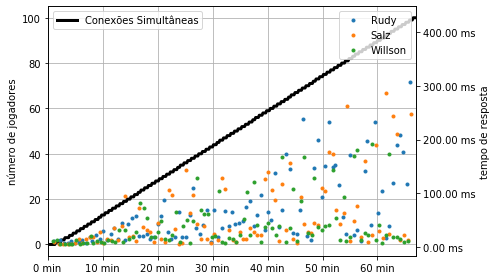
\includegraphics[width=0.8\textwidth]{figuras/analise/rt/start_session_request_time.png}
  \centering

  Fonte: O próprio autor.
\end{figure}

Tal qual as análises realizadas sobre as operações Criar Conta (Subseção~\ref{sec:op_create_account}) e Criar Personagem (Subseção~\ref{sec:op_create_char}), a Figura~\ref{fig:start_session_request_time} exibe o tempo de requisições que foram realizadas somente uma vez por cliente.
%
Os dados capturados mostram que o tempo de resposta segue uma tenência linear conforme o crescimento dos jogadores, diferente das outras operações.

A partir dessa diferença de comportamento, faz sentido analisar se existe algum crescimento, baseado na diluição destes dados a valores mais significativos para comparação.
%
Nesse contexto, faz sentido analisar o crescimento da média ao dividir as requisições em quadrantes.
%
Estes valores são exibidos na Tabela~\ref{tab:op_start_session}.

\begin{table}[htb!]
\centering
\begin{adjustbox}{max width=\textwidth}
\caption{Tempo de resposta médio dos quadrantes.}
\label{tab:op_start_session}
\begin{tabular}{l|l|l|l}

\hline \hline

Quadrante & Rudy    & Salz    & Willson \\ \hline \hline

Primeiro  & 18,6 ms & 20,88 ms & 15,68 ms \\ \hline

Segundo   & 45,4 ms & 52,38 ms & 40,48 ms \\ \hline

Terceiro  & 86,92 ms & 70,88 ms & 55,04 ms \\ \hline

Quarto    & 113,24 ms & 57,04 ms & 55,48 ms \\ \hline \hline

\end{tabular}

\end{adjustbox}

Fonte: O próprio autor.
\end{table}

A Tabela~\ref{tab:op_start_session} exibe o comportamento de crescimento conforme o crescimento de número de usuários, entretanto a média no último quadrante não aumenta proporcionalmente como nos quadrantes anteriores.
%
Não se pode, dessa forma, dizer que o crescimento é linear.

Outra informação exibida na Tabela~\ref{tab:op_start_session} é que a arquitetura Salz diminui drasticamente a média do seu tempo de resposta no quarto quadrante.
%
Também existe uma redução, se comparado aos demais quadrantes, quando visualizado o crescimento do quarto quadrante da arquitetura Willson.
%
Nesse sentido, pode-se adicionar a variável de estabilidade da \ac{api} analisada.

Para realizar a análise de estabilidade, faz sentido buscar a variância dos dados de cada quadrante.
%
Dessa forma pode-se analisar se existe uma flutuação maior comparado aos quadrantes anteriores, mesmo com uma média próxima.
%
A Tabela~\ref{tab:op_start_session_var} exibe a variância dos quadrantes.


\begin{table}[htb!]
\centering
\begin{adjustbox}{max width=\textwidth}
\caption{Variância dos quadrantes na operação Iniciar Sessão.}
\label{tab:op_start_session_var}
\begin{tabular}{l|l|l|l}

\hline \hline

Quadrante & Rudy    & Salz    & Willson \\ \hline \hline

Primeiro  & 205,92 & 865,47 & 247,58 \\ \hline

Segundo   & 477,60 & 1138,57 & 960,09 \\ \hline

Terceiro  & 2785,59 & 4091,28 & 2307,08 \\ \hline

Quarto    & 4801,06 & 5192,71 & 3740,09 \\ \hline \hline

\end{tabular}

\end{adjustbox}

Fonte: O próprio autor.
\end{table}

A Tabela~\ref{tab:op_start_session_var} exibe a informação referente a variação dos dados nos quadrantes.
%
Dessa forma, pode-se afirmar que a variação aumenta conforme a carga do serviço.
%
Nesse sentido, a média não apresenta um comportamento linear.
%
Porém, pode-se observar um comportamento de crescimento linear a partir da variância.
%
Dessa forma, deduz-se a seguinte relação:

$$
  \overline{IniciarSessao_{s}} < \overline{IniciarSessao_{w}} <\overline{IniciarSessao_{r}}
$$

Na qual entende-se:

\begin{itemize}
 \item $\overline{IniciarSessao_{r}}$: Tempo de resposta médio da operação iniciar sessão na arquitetura Rudy;
 \item $\overline{IniciarSessao_{s}}$: Tempo de resposta médio da operação iniciar sessão na arquitetura Salz; e
 \item $\overline{IniciarSessao_{w}}$: Tempo de resposta médio da operação iniciar sessão na arquitetura. Willson;
\end{itemize}
%ccm 13

\subsubsection{Instanciar personagem}

A operação de instanciar personagem é efetuada sobre o protocolo \ac{tcp}/\ac{rpc}.
%
Nesta operação, o cliente envia um formulário em formato \ac{gob}, com informações de autenticação assinadas pelo serviço junto a informação de qual personagem deve ser instanciado no mundo virtual.
%
Os dados são validados e o personagem selecionado é instanciado no mundo.

\begin{figure}[htb!]
  \caption{Tempo de resposta para instanciar personagens}
  \label{fig:spawn_character_request_time}
  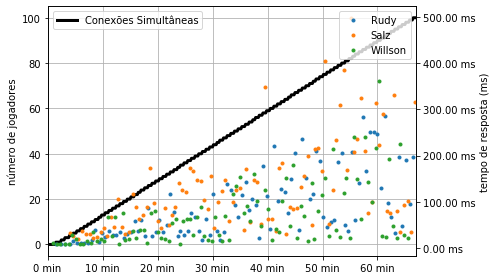
\includegraphics[width=0.8\textwidth]{figuras/analise/rt/spawn_character_request_time.png}
  \centering

  Fonte: O próprio autor.
\end{figure}

A Figura~\ref{fig:spawn_character_request_time} exibe o mesmo comportamento da operação iniciar sessão, abordada na Subseção~\ref{sec:op_start_session}.
%
Faz sentido aplicar os mesmos métodos para obter informações neste contexto, obtendo os valores de média e variância por quadrante.
%
Tais informações são exibidas na Tabela~\ref{tab:op_spawn_character}.

\begin{table}[htb!]
\centering
\begin{adjustbox}{max width=\textwidth}
\caption{Tempo de resposta médio e variância dos quadrantes para instanciar personagem.}
\label{tab:op_spawn_character}
\begin{tabular}{l||l|l||l|l||l|l}

\hline \hline

Quadrante & \multicolumn{2}{l||}{Rudy}    & \multicolumn{2}{l||}{Salz}    & \multicolumn{2}{l}{Willson} \\ \hline \hline

& Média & Variância & Média & Variância & Média & Variância \\ \hline

Primeiro  & 25,00 ms & 209,04 & 56,92 ms & 1350,23 & 24,64 ms & 368,15 \\ \hline

Segundo  & 59,12 ms & 1244,59 & 107,00 ms & 1617,25 & 42,24 ms & 8616,81 \\ \hline

Terceiro  & 123,00 ms & 3250,48 & 138,29 ms & 8661,54 & 86,72 ms & 2331,48 \\ \hline

Quarto  & 143,56 ms & 6984,89 & 202,12 ms & 14807,94 & 118,56 ms & 8616,81 \\ \hline \hline

\end{tabular}

\end{adjustbox}

Fonte: O próprio autor.
\end{table}

Diferente do comportamento da operação Iniciar Sessão (Subseção~\ref{sec:op_start_session}), ambos os comportamentos de variação e média exibidos na Tabela~\ref{tab:op_spawn_character} seguem um comportamento linear.
%
Deduz-se dessa forma que:

$$
  \overline{InstanciarPersonagem_{w}} < \overline{InstanciarPersonagem_{r}} <\overline{InstanciarPersonagem_{s}}
$$

Na qual entende-se:

\begin{itemize}
 \item $\overline{InstanciarPersonagem_{r}}$: Tempo de resposta médio da operação instanciar personagem na arquitetura Rudy;
 \item $\overline{InstanciarPersonagem_{s}}$: Tempo de resposta médio da operação instanciar personagem na arquitetura Salz; e
 \item $\overline{InstanciarPersonagem_{w}}$: Tempo de resposta médio da operação instanciar personagem na arquitetura Willson.
\end{itemize}


\subsubsection{Movimentar personagem}

A operação de movimentar personagem é efetuada sobre o protocolo \ac{tcp}/\ac{rpc}.
%
Nesta operação, o cliente envia um formulário em formato \ac{gob} com informações de autenticação assinadas pelo serviço junto a um vetor de direção para onde o personagem deve caminhar no mundo virtual.
%
Os dados são validados e o personagem instanciado é movimentado.

\begin{figure}[htb!]
  \caption{Tempo de resposta para movimentar personagens}
  \label{fig:move_character_request_time}
  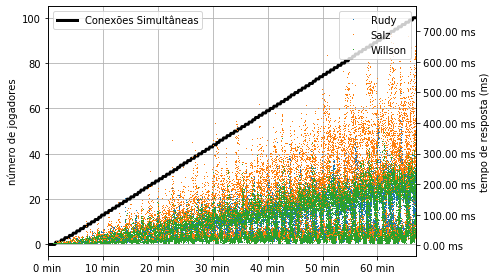
\includegraphics[width=0.8\textwidth]{figuras/analise/rt/move_character_request_time}
  \centering

  Fonte: O próprio autor.
\end{figure}

A Figura~\ref{fig:move_character_request_time} exibe os dados obtidos de tempo de resposta, esse tempo de resposta refere-se ao ato de movimentar o personagem durante a variação do número de jogadores simultâneos.
%
Percebe-se um gráfico denso, dada a quantidade de pontos obtidos neste experimento.
%
Dessa forma, faz sentido analisar o comportamento médio por jogador simultâneo.
%
A Figura~\ref{fig:spawn_character_request_time_per_concurrency} exibe o comportamento médio por jogador simultâneo.

\begin{figure}[htb!]
  \caption{Tempo médio de resposta para movimentar personagem comparado ao número de jogadores}
  \label{fig:spawn_character_request_time_per_concurrency}
  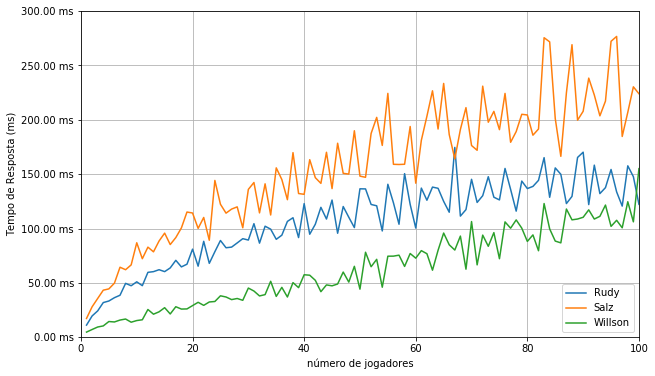
\includegraphics[width=0.8\textwidth]{figuras/analise/rt/spawn_character_request_time_per_concurrency}
  \centering

  Fonte: O próprio autor.
\end{figure}

Visivelmente, a Figura~\ref{fig:spawn_character_request_time_per_concurrency} permite deduzir dessa forma que:

$$
  \overline{MoverPersonagem_{w}} < \overline{MoverPersonagem_{r}} <\overline{MoverPersonagem_{s}}
$$

Assim, entende-se:

\begin{itemize}
 \item $\overline{MoverPersonagem_{r}}$: Tempo de resposta médio da operação mover personagem na arquitetura Rudy;
 \item $\overline{MoverPersonagem_{s}}$: Tempo de resposta médio da operação mover personagem na arquitetura Salz; e
 \item $\overline{MoverPersonagem_{w}}$: Tempo de resposta médio da operação mover personagem na arquitetura Willson.
\end{itemize}


\subsubsection{Enviar mensagem}

A operação de enviar mensagem é efetuada sobre o protocolo \ac{tcp}/\ac{rpc}.
%
Nesta operação, o cliente envia um formulário em formato \ac{gob} com informações de autenticação assinadas pelo serviço junto a uma linha de texto.
%
Os dados são validados e a linha de texto é distribuída aos personagens dentro do raio de visão do personagem emissor instanciado.

\begin{figure}[htb!]
  \caption{Tempo de resposta para enviar mensagens}
  \label{fig:send_chat_request_time}
  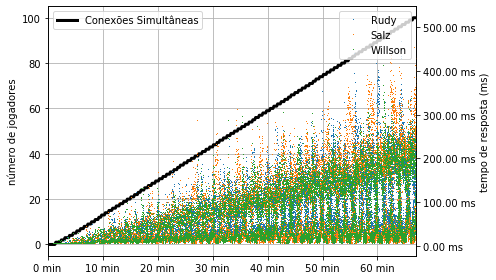
\includegraphics[width=0.8\textwidth]{figuras/analise/rt/send_chat_request_time}
  \centering

  Fonte: O próprio autor.
\end{figure}

A Figura~\ref{fig:send_chat_request_time} exibe os dados obtidos de tempo de resposta ao enviar uma mensagem no chat durante a variação do número de jogadores simultâneos.
%
Percebe-se um gráfico denso, dada a quantidade de pontos obtidos nos testes.
%
Dessa forma, faz sentido analisar o comportamento médio por jogador simultâneo.
%
A Figura~\ref{fig:send_chat_request_time_per_concurrency} exibe o comportamento médio por jogador simultâneo.


\begin{figure}[htb!]
  \caption{Tempo médio de resposta para enviar mensagens comparado ao número de jogadores simultâneos}
  \label{fig:send_chat_request_time_per_concurrency}
  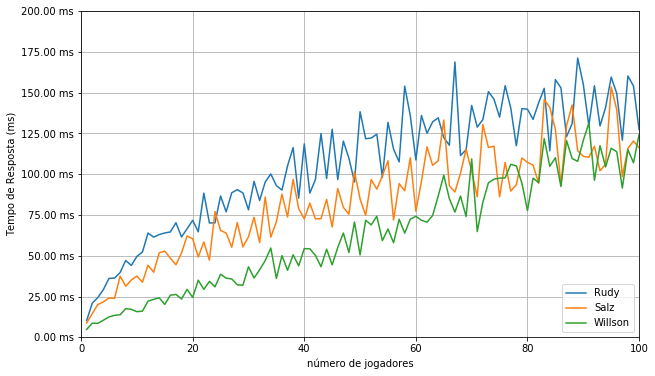
\includegraphics[width=0.8\textwidth]{figuras/analise/rt/send_chat_request_time_per_concurrency}
  \centering

  Fonte: O próprio autor.
\end{figure}

Visivelmente, a Figura~\ref{fig:send_chat_request_time_per_concurrency} permite deduzir dessa forma que:

$$
  \overline{EnviarMensagem_{w}} < \overline{EnviarMensagem_{s}} <\overline{EnviarMensagem_{r}}
$$

Deste modo, entende-se:

\begin{itemize}
 \item $\overline{EnviarMensagem_{r}}$: Tempo de resposta médio da operação enviar mensagem na arquitetura Rudy;
 \item $\overline{EnviarMensagem_{s}}$: Tempo de resposta médio da operação enviar mensagem na arquitetura Salz; e
 \item $\overline{EnviarMensagem_{w}}$: Tempo de resposta médio da operação enviar mensagem na arquitetura Willson.
\end{itemize}

\subsubsection{Receber mensagem}

A operação de receber mensagem é efetuada sobre o protocolo \ac{tcp}/\ac{rpc}.
%
Nesta operação, o cliente envia um formulário em formato \ac{gob} com informações de autenticação assinadas pelo serviço.
%
Os dados são validados e o serviço retorna todas as linhas de texto que foram encaminhadas ao personagem instanciado.

\begin{figure}[htb!]
  \caption{Tempo de resposta para receber mensagens}
  \label{fig:listen_chat_request_time}
  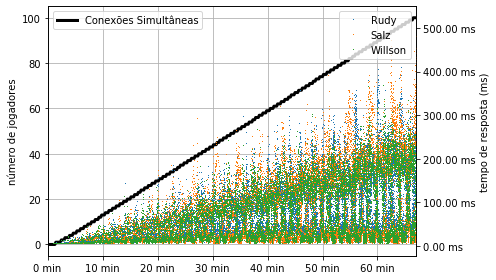
\includegraphics[width=0.8\textwidth]{figuras/analise/rt/listen_chat_request_time}
  \centering

  Fonte: O próprio autor.
\end{figure}

A Figura~\ref{fig:listen_chat_request_time} exibe os dados obtidos de tempo de resposta ao receber uma mensagem no chat, durante a variação do número de jogadores simultâneos.
%
Percebe-se um gráfico denso, dada a quantidade de pontos obtidos nos testes.
%
Dessa forma, faz sentido analisar o comportamento médio por jogador simultâneo.
%
A Figura~\ref{fig:listen_chat_request_time_per_concurrency} exibe o comportamento médio por jogador simultâneo.

\begin{figure}[htb!]
  \caption{Tempo médio de resposta para receber mensagens comparado ao número de jogadores}
  \label{fig:listen_chat_request_time_per_concurrency}
  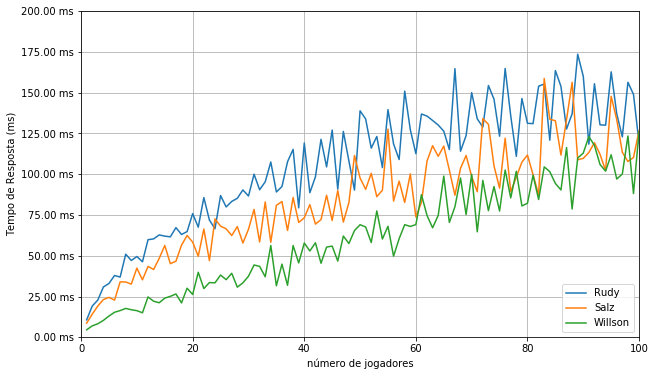
\includegraphics[width=0.8\textwidth]{figuras/analise/rt/listen_chat_request_time_per_concurrency}
  \centering

  Fonte: O próprio autor.
\end{figure}

Visivelmente, a Figura~\ref{fig:listen_chat_request_time_per_concurrency} permite deduzir dessa forma que:

$$
  \overline{ReceberMensagem_{w}} < \overline{ReceberMensagem_{s}} <\overline{ReceberMensagem_{r}}
$$

Logo, entende-se:

\begin{itemize}
 \item $\overline{ReceberMensagem_{r}}$: Tempo de resposta médio da operação receber mensagem na arquitetura Rudy;
 \item $\overline{ReceberMensagem_{s}}$: Tempo de resposta médio da operação receber mensagem na arquitetura Salz; e
 \item $\overline{ReceberMensagem_{w}}$: Tempo de resposta médio da operação receber mensagem na arquitetura Willson.
\end{itemize}

\subsection{Consumo de \ac{cpu}}

Este experimento visa analisar o consumo de \ac{cpu} unitariamente, em relação ao número de jogadores simultâneos.
%
Espera-se que o seu crescimento seja de tendência linear junto ao crescimento de jogadores concorrentes.
%
Neste contexto, existem as seguintes variáveis:

\begin{itemize}
    \item Jogadores simultâneos: Variável capturada a partir do microsserviço de jogo; e
    \item Consumo de \ac{cpu}: Variável capturada a partir do monitor de recursos do Docker.
\end{itemize}

Nota-se que o número de jogadores simultâneos e o consumo de \ac{cpu} são indexados pelo tempo a qual tais dados foram capturados.
%
Nesse sentido, pode-se relacionar o número de jogadores simultâneos ao consumo de \ac{cpu} dos microsserviços e do banco de dados.
%
Dado tal contexto, faz sentido realizar uma análise separando os ambientes de Banco de Dados de Microsserviços.

\subsubsection{Banco de Dados}

Considerando o ambiente de banco de dados, pode-se realizar a associação de número de jogadores simultâneos e \ac{cpu} consumida pelos contêineres de banco de dados.
%
Essa associação é realizada pelo tempo de registro das métricas.
%
O resultado desta associação pode ser visualizado na Figura~\ref{fig:experimento_db_cpu}.



\begin{figure}[htb!]
    \caption{Consumo de \ac{cpu} dos bancos de dados}
    \label{fig:experimento_db_cpu}

    \begin{subfigure}{0.5\textwidth}
        \centering
        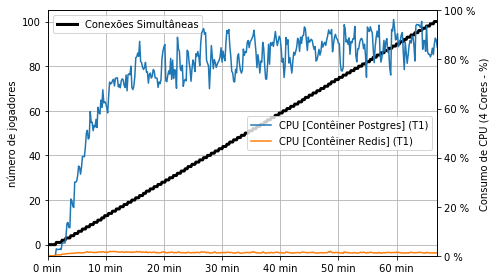
\includegraphics[width=.95\linewidth]{figuras/testes/r_cpu_db.png}
        \caption{Bancos de Dados da arquitetura Rudy}
        \label{fig:r_cpu_db}
    \end{subfigure}%
    \begin{subfigure}{0.5\textwidth}
        \centering
        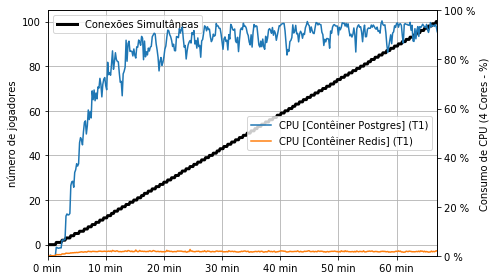
\includegraphics[width=.95\linewidth]{figuras/testes/s_cpu_db.png}
        \caption{Bancos de Dados da arquitetura Salz}
        \label{fig:s_cpu_db}
    \end{subfigure}\\

    \begin{subfigure}{0.5\textwidth}
        \centering
        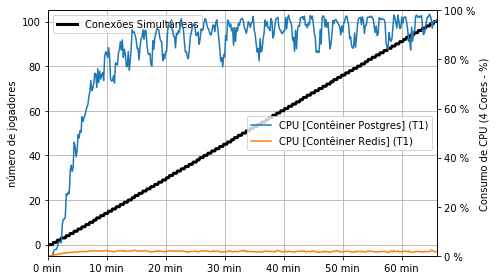
\includegraphics[width=.95\linewidth]{figuras/testes/w_cpu_db.png}
        \caption{Bancos de Dados da arquitetura Willson}
        \label{fig:w_cpu_db}
    \end{subfigure}

    Fonte: O próprio autor.
\end{figure}


A Figura~\ref{fig:experimento_db_cpu} exibe o comportamento do consumo de \ac{cpu} durante a execução dos testes para as arquiteturas Rudy (Subfigura~\ref{fig:r_cpu_db}), Salz (Subfigura~\ref{fig:s_cpu_db}) e Willson (Subfigura~\ref{fig:w_cpu_db}).
%
Em todas as figuras é notório o seguinte comportamento:

\begin{itemize}
 \item Baixo consumo de \ac{cpu} do servidor de dados temporários (Redis), com comportamento linear estável; e
 \item Alto consumo de \ac{cpu} do servidor de dados permanentes (PostgreSQL), com comportamento multimodal.
\end{itemize}

Este comportamento era esperado, dado a natureza distinta de ambos os banco de dados, na qual PostgreSQL é um banco de dados \ac{acid} e o Redis é um banco de dados \ac{nosql}.
%
Entretanto, é notório a discrepância entre ambos os bancos de dados, 
confirmando-se que o banco de dados temporário é estável em relação ao consumo de \ac{cpu}.

Ao analisar o comportamento do banco de dados persistentes para as arquiteturas Rudy (Subfigura~\ref{fig:r_cpu_db}), Salz (Subfigura~\ref{fig:s_cpu_db}) e Willson (Subfigura~\ref{fig:w_cpu_db}) observa-se um comportamento diferente na arquitetura Rudy.
%
Dada esta percepção, faz sentido analisar a tendência destas curvas com base em sua média.
%
A Tabela~\ref{tab:cpu_db_media_quadrantes} exibe os valores das médias baseado em todo o decorrer do experimento e dividindo o experimento em quadrantes.

\begin{table}[htb!]
\centering
\begin{adjustbox}{max width=\textwidth}
\caption{Consumo de \ac{cpu} por quadrante pelo PostgreSQL.}
\label{tab:cpu_db_media_quadrantes}
\begin{tabular}{l|l|l|l}

\hline \hline

Quadrante & Rudy    & Salz    & Willson \\ \hline \hline

Primeiro  & 50,60\% & 53,10\% & 58,15\% \\ \hline

Segundo   & 80,66\% & 88,04\% & 89,86\% \\ \hline

Terceiro  & 85,61\% & 90,77\% & 92,50\% \\ \hline

Quarto    & 86,94\% & 92,07\% & 93,48\% \\ \hline \hline

\end{tabular}

\end{adjustbox}

Fonte: O próprio autor.
\end{table}

Torna-se visível a diferença do consumo de \ac{cpu} entre as arquiteturas pelo banco de dados PostgreSQL.
%
A partir destes dados, pode-se deduzir que:

\begin{itemize}
 \item Arquitetura Rudy consome menos \ac{cpu} do banco de dados persistentes; e 
 \item Arquitetura Salz e Willson consomem \ac{cpu} na mesma proporção, com a arquitetura Salz tendo uma leve tendência a consumir menos \ac{cpu}.
\end{itemize}

Para tornar esta diferença visível ao longo de toda a progressão da carga, faz sentido exibir esta informação em um gráfico de linha.
%
A Figura~\ref{fig:cpu_db_media_por_jogador} exibe a média de consumo de \ac{cpu} pelo contêiner PostgreSQL comparado ao número de jogadores simultâneos.

\begin{figure}[htb!]
  \caption{Consumo de \ac{cpu} pelo PostgreSQL comparado ao número de jogadores simultâneos.}
  \label{fig:cpu_db_media_por_jogador}
  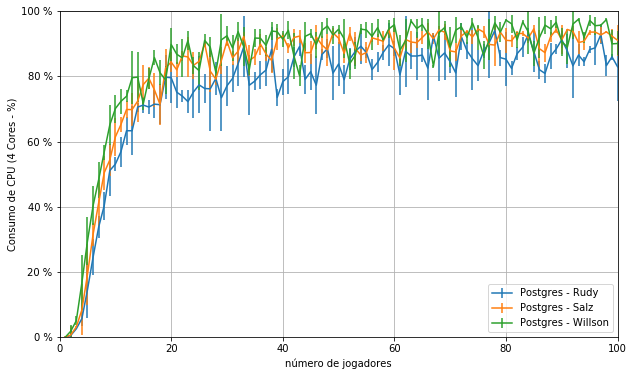
\includegraphics[width=0.8\textwidth]{figuras/analise/cpu_db_media_por_jogador.png}
  \centering

  Fonte: O próprio autor.
\end{figure}

Conforme exibido na Figura~\ref{fig:cpu_db_media_por_jogador}, pode-se deduzir que em todo caso as arquiteturas Rudy, Salz e Willson seguem a seguinte expressão:

$$
    CPU(db\_postgresql_{r}) < CPU(db\_postgresql_{s}) < CPU(db\_postgresql_{w})
$$

Logo, entende-se:

\begin{itemize}
\item $CPU(db\_postgresql_{r})$: Curva de consumo de \ac{cpu} pelo PostgreSQL da arquitetura Rudy;
\item $CPU(db\_postgresql_{s})$: Curva de consumo de \ac{cpu} pelo PostgreSQL da arquitetura Salz; e
\item $CPU(db\_postgresql_{w})$: Curva de consumo de \ac{cpu} pelo PostgreSQL da arquitetura Willson.
\end{itemize}

O banco de dados temporário consome pouca \ac{cpu}, comparado ao banco de dados persistente.
%
Entretanto, faz sentido realizar a mesma análise para validar se existe alguma diferença no seu uso conforme a arquitetura empregada.
%
Dessa forma, foi dividido em quadrantes para analisar o consumo médio de \ac{cpu}, a qual é exibido na Tabela~\ref{tab:cpu_redis_media_quadrantes}.

\begin{table}[htb!]
\centering
\begin{adjustbox}{max width=\textwidth}
\caption{Consumo de \ac{cpu} por quadrante pelo Redis.}
\label{tab:cpu_redis_media_quadrantes}
\begin{tabular}{|l|l|l|l|}

\hline

Quadrante & Rudy    & Salz    & Willson \\ \hline

Primeiro  & 1,24\% & 1,46\% & 1,60\% \\ \hline

Segundo   & 1,32\% & 1,79\% & 1,81\% \\ \hline

Terceiro  & 1,28\% & 1,75\% & 1,75\% \\ \hline

Quarto    & 1,26\% & 1,73\% & 1,72\% \\ \hline

\end{tabular}

\end{adjustbox}

Fonte: O próprio autor.
\end{table}

Dado os valores da Tabela~\ref{tab:cpu_redis_media_quadrantes}, pode-se obter as seguintes conclusões:

\begin{itemize}
 \item Rudy consome menos \ac{cpu} do banco de dados temporários; e
 \item A arquitetura Salz e Willson consomem \ac{cpu} com o mesmo comportamento.
\end{itemize}

Para tornar esta diferença visível ao longo de toda a progressão da carga, faz sentido exibir esta informação em um gráfico de linha.
%
A Figura~\ref{fig:cpu_redis_media_por_jogador} exibe um gráfico comparando a média de consumo de \ac{cpu} conforme o número de jogadores simultâneos.

\begin{figure}[htb!]
  \caption{Consumo de \ac{cpu} pelo PostgreSQL comparado ao número de jogadores simultâneos.}
  \label{fig:cpu_redis_media_por_jogador}
  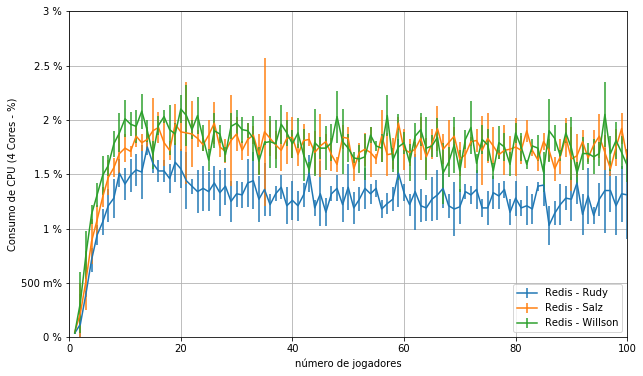
\includegraphics[width=0.8\textwidth]{figuras/analise/cpu_redis_media_por_jogador.png}
  \centering

  Fonte: O próprio autor.
\end{figure}

Conforme exibido na Figura~\ref{fig:cpu_redis_media_por_jogador}, pode-se deduzir que em todo caso as arquiteturas Rudy, Salz e Willson seguem a seguinte expressão:

$$
    CPU(db\_redis_{r}) < CPU(db\_redis_{s}) < CPU(db\_redis_{w})
$$

Na qual entende-se:

\begin{itemize}
\item $CPU(db\_redis_{r})$: Curva de consumo de \ac{cpu} pelo Redis da arquitetura Rudy;
\item $CPU(db\_redis_{s})$: Curva de consumo de \ac{cpu} pelo Redis da arquitetura Salz; e
\item $CPU(db\_redis_{w})$: Curva de consumo de \ac{cpu} pelo Redis da arquitetura Willson.
\end{itemize}

Nota-se que o consumo de recurso do banco de dados temporários e do banco de dados persistentes obtiveram o mesmo comportamento.
%
Dessa forma, pode-se generalizar o comportamento do consumo de \ac{cpu} das arquiteturas Rudy, Salz e Willson para o banco de Dados Redis:

$$
    CPU(db_{r}) < CPU(db_{s}) < CPU(db_{w})
$$

Na qual entende-se:

\begin{itemize}
\item $CPU(db_{r})$: Curva de consumo de \ac{cpu} pelos banco de dados da arquitetura Rudy;
\item $CPU(db_{s})$: Curva de consumo de \ac{cpu} pelos banco de dados da arquitetura Salz; e
\item $CPU(db_{w})$: Curva de consumo de \ac{cpu} pelos banco de dados da arquitetura Willson.
\end{itemize}

Este comportamento é dado pela característica do microsserviço \textit{rcrud} que realiza uma multiplexação de conexões entre o banco de dados e a arquitetura.
%
Entretanto, esta característica pode existir por dois motivos:

\begin{itemize}
 \item O banco de dados está otimizado para responder uma única conexão, consumindo menos \ac{cpu}; ou
 \item O banco de dados não consome tanta \ac{cpu} por ter um microsserviço que tornou-se um gargalo como frente do banco de dados.
\end{itemize}

Dado estas duas hipóteses, faz sentido mensurar a qualidade de serviço entregue ao usuário.
%
Pode-se mensurar qual das hipóteses é mais valiosa para a qualidade de serviço com base no tempo de resposta do usuário.


\subsubsection{Microsserviços}

Considerando o ambiente de banco de dados, pode-se realizar a associação de número de jogadores simultâneos e \ac{cpu} consumida pelos contêineres de banco de dados.
%
Essa associação é realizada pelo tempo de registro das métricas.
%
O resultado desta associação pode ser visualizado na Figura~\ref{fig:experimento_game_cpu}.

\begin{figure}[htb!]
    \caption{Consumo de \ac{cpu} dos microsserviços}
    \label{fig:experimento_game_cpu}

    \begin{subfigure}{0.5\textwidth}
        \centering
        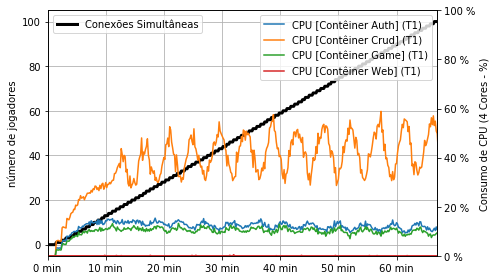
\includegraphics[width=.95\linewidth]{figuras/testes/r_cpu_game.png}
        \caption{Microsserviços da arquitetura Rudy}
        \label{fig:r_cpu_game}
    \end{subfigure}%
    \begin{subfigure}{0.5\textwidth}
        \centering
        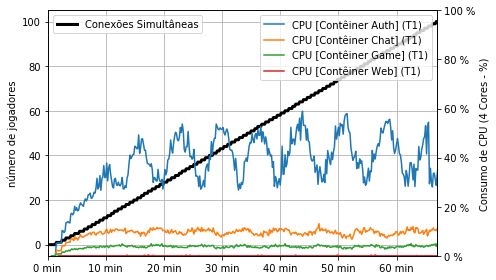
\includegraphics[width=.95\linewidth]{figuras/testes/s_cpu_game.png}
        \caption{Microsserviços da arquitetura Salz}
        \label{fig:s_cpu_game}
    \end{subfigure}

    \begin{subfigure}{0.5\textwidth}
        \centering
        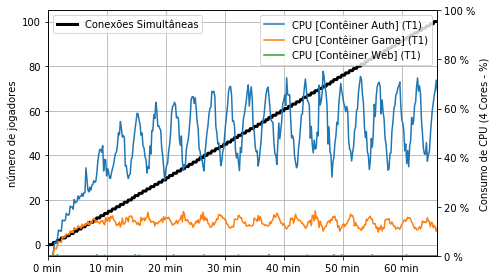
\includegraphics[width=.95\linewidth]{figuras/testes/w_cpu_game.png}
        \caption{Microsserviços da arquitetura Willson}
        \label{fig:w_cpu_game}
    \end{subfigure}%

    Fonte: O próprio autor.
\end{figure}

Conforme exibido nas Figuras~\ref{fig:r_cpu_game}, ~\ref{fig:s_cpu_game} e ~\ref{fig:w_cpu_game}, pode-se observar as seguintes características:

\begin{itemize}
 \item Os microsserviços \textit{rweb}, \textit{sweb} e \textit{wweb} consomem pouca \ac{cpu} comparados a todos os outros microsserviços das arquiteturas; e
 \item Os microsserviços \textit{rcrud}, \textit{sauth} e \textit{wauth} são os microsserviços que mais consomem \ac{cpu} nas arquiteturas Rudy, Salz e Willson respectivamente.
\end{itemize}

Faz sentido analisar a média do consumo de \ac{cpu} dos microsserviços dividindo em quadrantes.
%
Dessa forma, pode-se obter dados significantes para realizar comparações a partir destes dados.
%
A Tabela~\ref{tab:cpu_microsservicos_media_quadrantes} exibe a média de consumo de \ac{cpu} por quadrante de todos os microsserviços.

\begin{table}[htb!]
\centering
\begin{adjustbox}{max width=\textwidth}
\caption{Consumo de \ac{cpu} por quadrante dos microsserviços.}
\label{tab:cpu_microsservicos_media_quadrantes}

\begin{tabular}{l|l|l|l|l}
\hline \hline
Microsserviço & Primeiro Quadrante & Segundo Quadrante & Terceiro Quadrante & Quarto Quadrante \\ \hline \hline
rauth         & 11,22\%            & 12,52\%           & 11,88\%            & 11,56\%          \\ \hline
rcrud         & 25,97\%            & 41,83\%           & 42,50\%             & 43,62\%          \\ \hline
rgame         & 8,92\%             & 10,54\%           & 10,14\%            & 9,58\%           \\ \hline
rweb          & 0,01\%             & 0,01\%            & 0,01\%             & 0,01\%           \\ \hline
sauth         & 26,08\%            & 39,95\%           & 43,22\%            & 40,96\%          \\ \hline
schat         & 8,34\%             & 9,97\%            & 9,59\%             & 9,61\%           \\ \hline
sgame         & 3,12\%             & 3,87\%            & 3,72\%             & 3,85\%           \\ \hline
sweb          & 0,01\%             & 0,01\%            & 0,01\%             & 0,01\%           \\ \hline
wauth         & 23,79\%            & 50,73\%           & 57,11\%            & 56,69\%          \\ \hline
wgame         & 9,68\%             & 14,20\%           & 13,66\%            & 13,42\%          \\ \hline
wweb          & 0,01\%             & 0,01\%            & 0,01\%             & 0,01\%           \\ \hline \hline
\end{tabular}
\end{adjustbox}

Fonte: O próprio autor.
\end{table}

A Tabela~\ref{tab:cpu_microsservicos_media_quadrantes} mostra o crescimento do consumo de carga médio dos quadrantes.
%
Estes dados são importantes, haja vista que os mesmos permitem analisar o comportamento das curvas removendo oscilações notórias na visualização do consumo de \ac{cpu}.
%
A partir da Tabela~\ref{tab:cpu_microsservicos_media_quadrantes}, pode-se realizar as seguintes conclusões:

\begin{itemize}
 \item Entre os microsserviços \textit{rcrud}, \textit{sauth} e \textit{wauth}, o com maior consumo é o microsserviço \textit{wauth}; e
 \item Os microsserviços \textit{rweb}, \textit{sweb} e \textit{wweb} possuem o mesmo consumo em média.
\end{itemize}

É relevante, a partir destas conclusões, analisar a média em relação a progressão de usuários.
%
A visualização da média de consumo de \ac{cpu} por usuário simultâneo tem como objetivo remover ruídos que possam afetar a visualização dos dados.

\begin{figure}[htb!]
    \caption{Média do consumo de \ac{cpu} dos microsserviços por jogador simultâneo}
    \label{fig:cpu_game_media_por_jogador}

    \begin{subfigure}{0.5\textwidth}
        \centering
        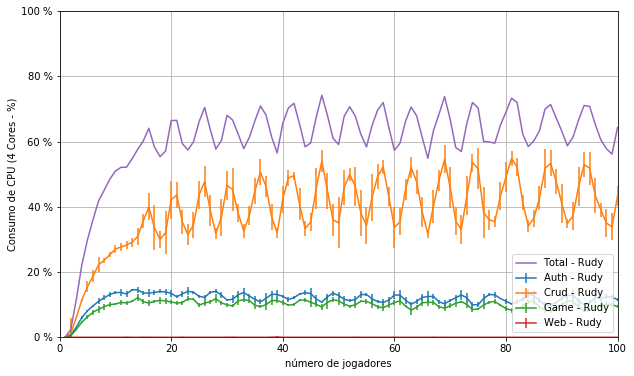
\includegraphics[width=.95\linewidth]{figuras/analise/cpu_r_arch_media_por_jogador.png}
        \caption{Microsserviços da arquitetura Rudy}
        \label{fig:cpu_r_arch_media_por_jogador}
    \end{subfigure}%
    \begin{subfigure}{0.5\textwidth}
        \centering
        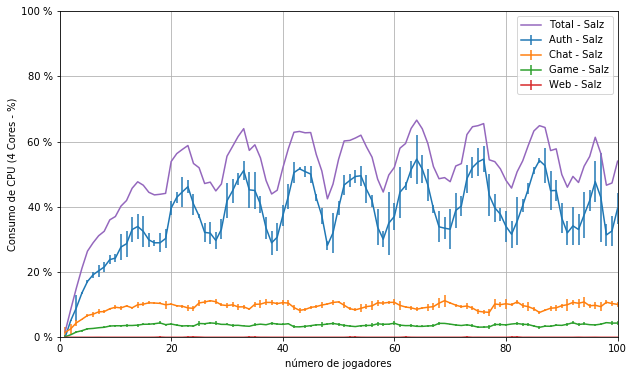
\includegraphics[width=.95\linewidth]{figuras/analise/cpu_s_arch_media_por_jogador.png}
        \caption{Microsserviços da arquitetura Salz}
        \label{fig:cpu_s_arch_media_por_jogador}
    \end{subfigure}

    \begin{subfigure}{0.5\textwidth}
        \centering
        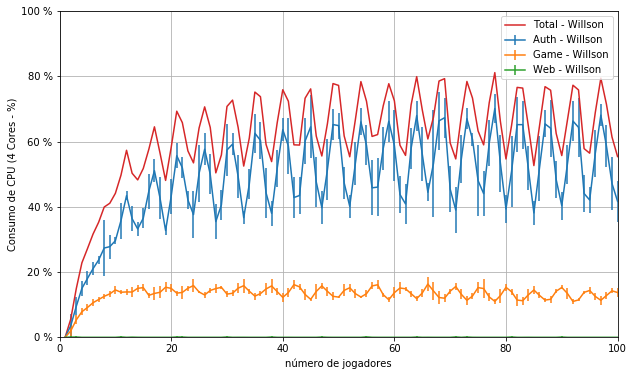
\includegraphics[width=.95\linewidth]{figuras/analise/cpu_w_arch_media_por_jogador.png}
        \caption{Microsserviços da arquitetura Willson}
        \label{fig:cpu_w_arch_media_por_jogador}
    \end{subfigure}%

    Fonte: O próprio autor.
\end{figure}

A Figura~\ref{fig:cpu_game_media_por_jogador} tem como objetivo exibir a média de consumo de \ac{cpu} por jogador, assim permitindo analisar o comportamento das curvas.
%
Entretanto, nota-se que todos os microsserviços contém uma característica senoidal, na qual sua amplitude aumenta com a quantidade de jogadores, característa essa que já era visível na Figura~\ref{fig:experimento_game_cpu}.
%
Porém, neste gráfico também é visível o erro de cada média.
%
Este erro é dado pela variância do conjunto de dados obtidos na determinada faixa de jogadores simultâneos.
%
Ter um valor de variância alto significa que, por mais que a média seja um bom valor para a métrica, diversos pontos da mesma faixa estão longe do valor médio.
%
Dessa forma, pode-se interpretar como uma quantificação de variação ou como uma margem de erro, neste contexto.

Pode-se deduzir as seguintes características a partir da Figura~\ref{fig:cpu_game_media_por_jogador}:

\begin{itemize}
 \item Os microsserviços que contém maior margem de erro são os que estão relacionados a acesso de dados para autenticação e/ou geração de assinaturas de dados para outros serviços (\textit{rcrud, sauth e wauth});
 \item Os microsserviços que contém maior margem de erro, são os que lideram a lista de maior consumo de \ac{cpu}, porém nota-se a partir dos demais microsserviços que esta relação não é proporcional a carga; e
 \item O valor total de consumo de \ac{cpu} muda conforme a arquitetura.
\end{itemize}

Dado o último critério, utilizando a curva de total consumido das Subfiguras~\ref{fig:cpu_r_arch_media_por_jogador}, ~\ref{fig:cpu_s_arch_media_por_jogador} e ~\ref{fig:cpu_w_arch_media_por_jogador},  pode-se comparar o total de consumo de \ac{cpu} por cada arquitetura.
%
A Tabela~\ref{tab:consumo_total_cpu} exibe os valores baseados em quadrantes, para realizar a comparação com valores.


\begin{table}[htb!]
\centering
\begin{adjustbox}{max width=\textwidth}
\caption{Consumo total de \ac{cpu} por quadrante dos microsserviços.}
\label{tab:consumo_total_cpu}

\begin{tabular}{l|l|l|l|l}
\hline \hline
Arquitetura & Primeiro Quadrante & Segundo Quadrante & Terceiro Quadrante & Quarto Quadrante \\ \hline \hline
Rudy        & 47,05\%            & 64,51\%           & 65,25\%            & 64,31\%          \\ \hline
Salz        & 38,74\%            & 53,87\%           & 56,74\%            & 54,27\%          \\ \hline
Willson     & 44,60\%            & 65,76\%           & 67,94\%            & 66,98\%          \\ \hline \hline
\end{tabular}
\end{adjustbox}

Fonte: O próprio autor.
\end{table}

A partir dos dados da Tabela~\ref{tab:consumo_total_cpu}, pode-se referenciar que a arquitetura Salz consome menos \ac{cpu} que a arquitetura Rudy e Willson.
%
Faz sentido realizar a visualização das três curvas de totais em um único gráfico, a fim de exibir esta relação identificada.
%
A Figura~\ref{fig:consumo_total_cpu} exibe esta comparação.

\begin{figure}[htb!]
  \caption{Comparação de consumo total de \ac{cpu} pelas arquiteturas.}
  \label{fig:consumo_total_cpu}
  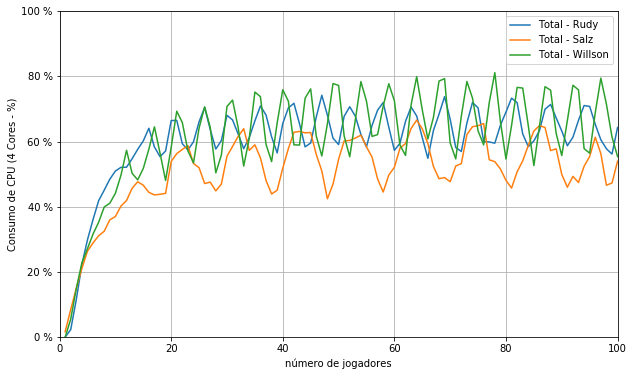
\includegraphics[width=0.8\textwidth]{figuras/analise/cpu_total_archs.png}
  \centering

  Fonte: O próprio autor.
\end{figure}

Dado a Figura~\ref{fig:consumo_total_cpu} e a Tabela~\ref{tab:consumo_total_cpu}, pode-se afirmar que:

$$
    CPU(microsservicos_{s}) < CPU(microsservicos_{r}) < CPU(microsservicos_{w})
$$

Na qual entende-se:

\begin{itemize}
\item $CPU(microsservicos_{r})$: Curva de consumo de \ac{cpu} pelos microsserviços da arquitetura Rudy;
\item $CPU(microsservicos_{s})$: Curva de consumo de \ac{cpu} pelos microsserviços da arquitetura Salz; e
\item $CPU(microsservicos_{w})$: Curva de consumo de \ac{cpu} pelos microsserviços da arquitetura Willson.
\end{itemize}

Torna-se notório que tal sequência respeita a ordem de interconexões dos microsserviços.
%
Nesse sentido, a arquitetura Salz possui mais conexões que a arquitetura Rudy, que possui mais conexões que a arquitetura Willson.

Nota-se que possuir um consumo de \ac{cpu} maior que outra arquitetura não implica em ser uma arquitetura melhor.
%
Pode-se encontrar dois casos para um consumo de \ac{cpu} menor ao comparar duas arquiteturas:

\begin{itemize}
 \item A arquitetura que consome menos \ac{cpu} possui pouca carga para estressá-la; ou
 \item A arquitetura que consome menos \ac{cpu} converge para tal valor, visto que está com gargalo em outro recurso necessário.
\end{itemize}

Para o caso desta análise, pode-se descartar a primeira alternativa.
%
Com isso, pode-se analisar que a curva estabiliza o seu crescimento entre 20 e 40 jogadores simultâneos, a mesma faixa na qual os bancos de dados estabilizaram seu crescimento (visível na Figura~\ref{fig:cpu_db_media_por_jogador}).
%
Dessa forma, torna-se justificável o aumento da margem de erro nas médias dos microsserviços com acesso ao banco conforme o aumento da carga no serviço.

Outra característica das curvas obtidas é a frequência da oscilação encontrada, característica visível na Figura~\ref{fig:experimento_game_cpu}.
%
Nota-se que a frequência é escalada tal qual a crista de uma onda entra em contato com o vale da outra onda.
%
Tal característica das curvas não é coincidência, sendo possivelmente um resultado do escalonador de contêineres.
%
A Figura~\ref{fig:cpu_w_arch_media_por_jogador} é a que melhor exemplifica este comportamento, haja vista que a arquitetura Willson possui somente dois microsserviços que são impactados diretamente por este escalonador.


\subsection{Consumo de Memória}



Este experimento visa analisar o consumo de memória unitariamente, em relação ao número de jogadores simultâneos.
%
Espera-se que o seu crescimento seja linear seguindo o crescimento de jogadores concorrentes.
%
Neste contexto existem os seguintes valores:



\begin{itemize}
    \item Jogadores simultâneos: Variável capturada a partir do microsserviço de jogo; e
    \item Consumo de memória: Variável capturada a partir do monitor de recursos do Docker.
\end{itemize}

Nota-se que o número de jogadores simultâneos e o consumo de memória são indexados pelo tempo a qual tais dados foram capturados.
%
Nesse sentido, pode-se relacionar, o número de jogadores simultâneos ao consumo de memória dos microsserviços e do banco de dados.
%
Dado tal contexto, faz sentido realizar uma análise separando os ambientes de Banco de Dados de Microsserviços.

\subsubsection{Banco de Dados}



Considerando o ambiente de banco de dados, pode-se realizar a associação do número de jogadores simultâneos e a memória consumida pelos contêineres de banco de dados.
%
Essa associação é realizada pelo tempo de registro das métricas.
%
O resultado desta associação pode ser visualizado na Figura~\ref{fig:experimento_db_mem}.



\begin{figure}[htb!]
    \caption{Consumo de memória dos bancos de dados}
    \label{fig:experimento_db_mem}

    \begin{subfigure}{0.5\textwidth}
        \centering
        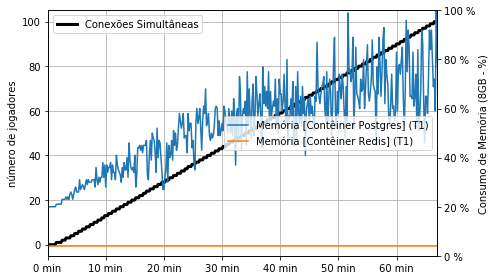
\includegraphics[width=.95\linewidth]{figuras/testes/r_mem_db.png}
        \caption{Bancos de Dados da arquitetura Rudy}
        \label{fig:r_mem_db}
    \end{subfigure}%
    \begin{subfigure}{0.5\textwidth}
        \centering
        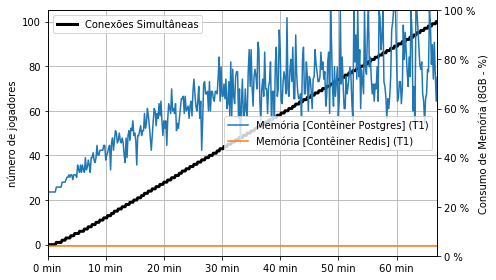
\includegraphics[width=.95\linewidth]{figuras/testes/s_mem_db.png}
        \caption{Bancos de Dados da arquitetura Salz}
        \label{fig:s_mem_db}
    \end{subfigure}\\

    \begin{subfigure}{0.5\textwidth}
        \centering
        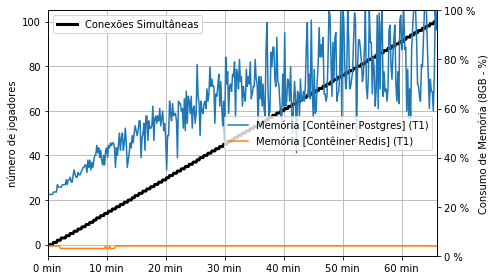
\includegraphics[width=.95\linewidth]{figuras/testes/w_mem_db.png}
        \caption{Bancos de Dados da arquitetura Willson}
        \label{fig:w_mem_db}
    \end{subfigure}

    Fonte: O próprio autor.
\end{figure}

Percebe-se, a partir da Figura~\ref{fig:experimento_db_mem}, que o banco de daados com maior estresse é o PostgreSQL.
%
O banco de dados Redis consome uma quantidade de memória visivelmente constante.
%
Entretanto, o banco de dados Redis é utilizado para armazenamento de dados da sessão do cliente em memória.
%
Assim, faz sentido calcular a quantidade de memória consumida por cada usuário para garantir que na totalidade este valor não é significativo em porcentagem.

Para realizar a autenticação é utilizado uma chave de valores aleatórios.
%
Contudo, é necessário garantir uma única conexão por usuário.
%
A unicidade é realizada utilizando o Redis, armazenando uma sequência de caracteres aleatórias em um campo formatado com o nome do usuário.
%
O trecho de código que realiza esta operação é exibido na Listagem~\ref{lst:seq_chars_redis}.



\begin{lstlisting}[language=go,firstnumber=1, caption={Informações do Bloco},label={lst:seq_chars_redis}]
package merepositories

// mmosandbox/infra/merepositories/token_repositoriy.go

// GenerateToken based in username from account
func (repository *TokenRepository) GenerateToken(username string) string {
    token := repository.randomToken()
    repository.set(repository.keyPattern(username), token)

    return token
}

// keyPattern to store into redis
func (repository *TokenRepository) keyPattern(username string) string {
    return fmt.Sprintf("session.%s", username)
}

// randomToken with 256 runes
func (repository *TokenRepository) randomToken() string {
    return randomize.RandStringRunes(256)
}
\end{lstlisting}

O repositório de dados \textit{TokenRepository}\footnote{\textit{TokenRepository}: \url{https://github.com/schweigert/mmosandbox/blob/master/infra/merepositories/token_repositoriy.go}} contém as operações exibidas na Listagem~\ref{lst:seq_chars_redis}.
%
Este repositório gera a chave com o padrão \textit{session.\%s} e uma sequência de caracteres aleatória de 256 bytes.

Para realizar este calculo é necessário estimar o custo de armazenamento das chaves.
%
Por padrão, os clientes de ataque geram nomes de usuários de 32 caracteres.
%
Com tais dados pode-se estimar o custo de memória por usuário utilizando a seguinte fórmula:

\begin{multline}
m_j = m_{chave} + m_{padrao} + m_{valor} \\
\Rightarrow m_j = 32bytes + 8bytes + 256bytes = 296bytes
\end{multline}

Sendo que:

\begin{itemize}
\item $m_j$: Tamanho dos dados armazenados em memória no Redis por jogador autenticado;
\item $m_{chave}$: Tamanho da chave armazenada na estrutura chave-valor Redis; e
\item $m_{valor}$: Tamanho do valor armazenado na estrutura chave-valor do Redis.
\end{itemize}


Logo, ao ter 100 jogadores simultâneos, o serviço Redis consumirá aproximadamente 29Kb para armazenamento de memória.
%
Tal valor é insignificante comparado ao total de memória disponível no hospedeiro, dessa forma exibindo um comportamento retilíneo na Figura~\ref{fig:experimento_db_mem}.

Entretanto, o PostgreSQL exibe um crescimento linear visível na Figura~\ref{fig:experimento_db_mem}.
%
Faz sentido sanitizar estas curvas com a média dos quadrantes.
%
A Tabela~\ref{tab:mem_db_media_quadrantes} exibe o consumo de memória médio por quadrante.

\begin{table}[htb!]
\centering
\begin{adjustbox}{max width=\textwidth}
\caption{Consumo médio de memória por quadrante do PostgreSQL.}
\label{tab:mem_db_media_quadrantes}

\begin{tabular}{l|l|l|l|l}
\hline \hline
Arquitetura & Primeiro Quadrante & Segundo Quadrante & Terceiro Quadrante & Quarto Quadrante \\ \hline \hline
Rudy        & 32,41\%            & 54,07\%           & 65,92\%            & 73,57\%          \\ \hline
Salz        & 39,56\%            & 61,52\%           & 71,84\%            & 76,29\%          \\ \hline
Willson     & 38,83\%            & 61,72\%           & 72,43\%            & 79,25\%          \\ \hline \hline
\end{tabular}
\end{adjustbox}

Fonte: O próprio autor.
\end{table}

A partir da Tabela~\ref{tab:mem_db_media_quadrantes}, pode-se mensurar a diferença de consumo de memória pelas arquiteturas consumidas pelo PostgreSQL.
%
No quarto quadrante observa-se uma diferença no consumo, médio, conforme a arquitetura empregada.=
%
Entretanto, não se pode mensurar que existe uma tendência, visto que o segundo e terceiro quadrante ficam próximos.
%
Dado tais informações pode-se parcialmente concluir que o consumo de memória por parte do banco de dados persistentes é menor na arquitetura Rudy.
%
Contudo, o consumo é demasiadamente próximo entre as arquiteturas Willson e Salz, tendo a arquitetura Salz uma leve tendência a ser maior.

Tal comportamento faz sentido, levando em consideração o número de conexões simultâneas que cada arquitetura realiza ao banco de dados.
%
A arquitetura Rudy contém poucas conexões simultâneas ao banco de dados persistentes, haja vista que concentra todas suas conexões ao microsserviço \textit{rcrud}, o qual ocorre a partir de todos os microsserviços das demais arquiteturas.

Para corroborar esta conclusão, faz sentido correlacionar a média de consumo de memória pelo banco de dados persistentes correlacionado ao número de jogadores simultâneos.
%
Tal correlação é visível na Figura~\ref{fig:mem_db_media_por_jogador}.

\begin{figure}[htb!]
  \caption{Consumo de memória média do PostgreSQL comparado ao número de jogadores simultâneos.}
  \label{fig:mem_db_media_por_jogador}
  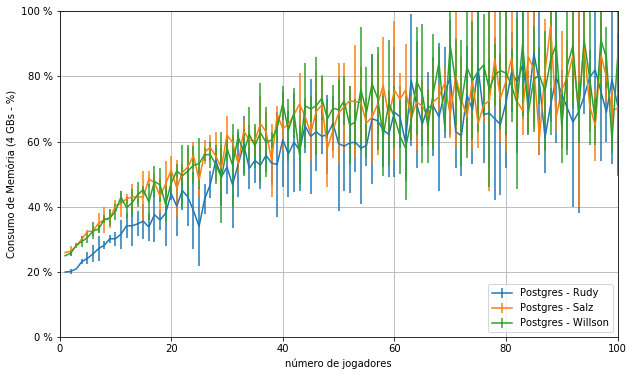
\includegraphics[width=0.8\textwidth]{figuras/analise/mem_db_media_por_jogador.png}
  \centering

  Fonte: O próprio autor.
\end{figure}

A partir da Figura~\ref{fig:mem_db_media_por_jogador} pode-se confirmar as conclusões parciais obtidas da Tabela~\ref{tab:cpu_db_media_quadrantes}.
%
Além das conclusões parciais, é possível visualizar o crescimento da média a cada incremento de jogador simultâneo.
%
Sendo assim, pode-se concluir que o serviço de banco de dados PostgreSQL de fato foi estressado, haja vista que pode-se perceber inicialmente um comportamento na qual não corresponde a uma curva multimodal.

A partir destes dados conclui-se que:

$$
    MEM(db\_postgresql_{r}) < MEM(db\_postgresql_{s}) \approx MEM(db\_postgresql_{w})
$$

Na qual entende-se:

\begin{itemize}
\item $MEM(db\_postgresql_{r})$: Curva de consumo de memória do PostgreSQL pela arquitetura Rudy;
\item $MEM(db\_postgresql_{s})$: Curva de consumo de memória do PostgreSQL pela arquitetura Salz; e
\item $MEM(db\_postgresql_{w})$: Curva de consumo de memória do PostgreSQL pela arquitetura Willson.
\end{itemize}


\subsubsection{Microsserviços}

Considerando o ambiente de microsserviços, pode-se realizar a associação de número de jogadores simultâneos e memória consumida pelos contêineres de banco de dados.
%
Essa associação é realizada pelo tempo de registro das métricas.
%
O resultado desta associação pode ser visualizado na Figura~\ref{fig:experimento_gs_mem}.


\begin{figure}[htb!]
    \caption{Consumo de memória dos microsserviços}
    \label{fig:experimento_gs_mem}

    \begin{subfigure}{0.5\textwidth}
        \centering
        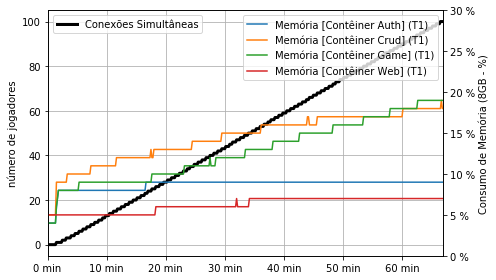
\includegraphics[width=.95\linewidth]{figuras/testes/r_mem_game.png}
        \caption{Microsserviço da arquitetura Rudy}
        \label{fig:r_mem_game}
    \end{subfigure}%
    \begin{subfigure}{0.5\textwidth}
        \centering
        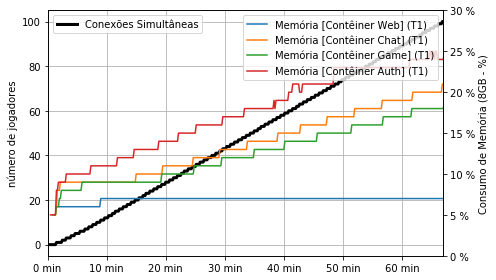
\includegraphics[width=.95\linewidth]{figuras/testes/s_mem_game.png}
        \caption{Microsserviço da arquitetura Salz}
        \label{fig:s_mem_game}
    \end{subfigure}\\

    \begin{subfigure}{0.5\textwidth}
        \centering
        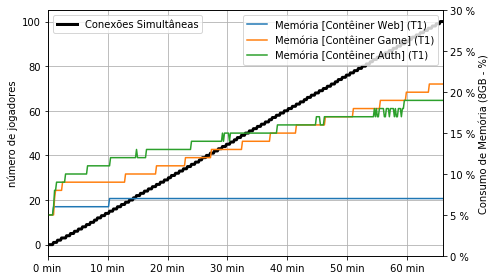
\includegraphics[width=.95\linewidth]{figuras/testes/w_mem_game.png}
        \caption{Microsserviço da arquitetura Willson}
        \label{fig:w_mem_game}
    \end{subfigure}

    Fonte: O próprio autor.
\end{figure}

Ao escalar os jogadores simultâneos no serviço, a memória consumida pelas arquiteturas de microsserviços cresce linearmente, com alguns saltos.
%
Tais saltos, visíveis na Figura~\ref{fig:experimento_gs_mem}, são provenientes do gerenciador de memória da linguagem de implementação.
%
Este método de alocação de memória tenta evitar a comunicação com o sistema operacional para esta alocação de memória.


Faz sentido analisar o comportamento em quadrantes, já que o seu crescimento é linear.
%
Dessa forma podemos analisar o comportamento de crescimento dos microsserviços e realizar uma análise comparativa sobre os dados obtidos.
%
Pode-se visualizar estes dados na Tabela~\ref{tab:mem_gs_media}.

\begin{table}[htb!]
\centering
\begin{adjustbox}{max width=\textwidth}
\caption{Consumo médio de memória pelos microsserviços.}
\label{tab:mem_gs_media}

\begin{tabular}{l|l|l|l|l|l|l|l|l}
\hline
\hline
\multirow{2}{*}{Microsserviços} & \multicolumn{2}{l|}{Quadrante 1} & \multicolumn{2}{l|}{Quadrante 2} & \multicolumn{2}{l|}{Quadrante 3} & \multicolumn{2}{l}{Quadrante 4} \\ \cline{2-9} 
                                & Média  & Total                   & Média  & Total                   & Média  & Total                   & Média  & Total                   \\ \hline \hline
rauth                           & 8 \%   & \multirow{4}{*}{33 \%}  & 9 \%   & \multirow{4}{*}{41 \%}  & 9 \%   & \multirow{4}{*}{49 \%}  & 9 \%   & \multirow{4}{*}{53 \%}  \\ \cline{1-2} \cline{4-4} \cline{6-6} \cline{8-8}
rcrud                           & 11 \%  &                         & 14 \%  &                         & 17 \%  &                         & 18 \%  &                         \\ \cline{1-2} \cline{4-4} \cline{6-6} \cline{8-8}
rgame                           & 9 \%   &                         & 12 \%  &                         & 16 \%  &                         & 19 \%  &                         \\ \cline{1-2} \cline{4-4} \cline{6-6} \cline{8-8}
rweb                            & 5 \%   &                         & 6 \%   &                         & 7 \%   &                         & 7 \%   &                         \\ \hline \hline
sauth                           & 9 \%   & \multirow{4}{*}{34 \%}  & 12 \%  & \multirow{4}{*}{41 \%}  & 16 \%  & \multirow{4}{*}{51 \%}  & 19 \%  & \multirow{4}{*}{60 \%}  \\ \cline{1-2} \cline{4-4} \cline{6-6} \cline{8-8}
schat                           & 9 \%   &                         & 11 \%  &                         & 14 \%  &                         & 17 \%  &                         \\ \cline{1-2} \cline{4-4} \cline{6-6} \cline{8-8}
sgame                           & 9 \%   &                         & 11 \%  &                         & 14 \%  &                         & 17 \%  &                         \\ \cline{1-2} \cline{4-4} \cline{6-6} \cline{8-8}
sweb                            & 7 \%   &                         & 7 \%   &                         & 7 \%   &                         & 7 \%   &                         \\ \hline \hline
wauth                           & 10 \%  & \multirow{3}{*}{26 \%}  & 12 \%  & \multirow{3}{*}{31 \%}  & 16 \%  & \multirow{3}{*}{39 \%}  & 20 \%  & \multirow{3}{*}{47 \%}  \\ \cline{1-2} \cline{4-4} \cline{6-6} \cline{8-8}
wgame                           & 9 \%   &                         & 12 \%  &                         & 16 \%  &                         & 20 \%  &                         \\ \cline{1-2} \cline{4-4} \cline{6-6} \cline{8-8}
wweb                            & 7 \%   &                         & 7 \%   &                         & 7 \%   &                         & 7 \%   &                         \\ \hline \hline
\end{tabular}
\end{adjustbox}

Fonte: O próprio autor.
\end{table}

A partir da Tabela~\ref{tab:mem_gs_media} podemos deduzir diversas características dos microsserviços e das arquiteturas.
%
Dessa forma, deduz-se sobre os microsserviços que:

\begin{itemize}
 \item Ao comparar os microsserviços de autenticação, percebe-se que o microsserviço \textit{rauth} não aumenta o seu consumo de memória, repassando o seu consumo de memória ao microsserviço \textit{rcrud};
 \item O microsserviço \textit{rweb} consome menos memória comparado aos microsserviços \textit{sweb} e \textit{wweb} pois não realiza conexão com o banco de dados; e
 \item Os microsserviços \textit{schat} e \textit{sgame} consomem menos memória ao comparar com os microsserviços \textit{wgame} e \textit{rgame}, individualmente. Entretanto a soma dos microsserviços \textit{schat} e \textit{sgame} consome mais memória que os microsserviços \textit{wgame} e \textit{rgame}, individualmente.
\end{itemize}

A partir do consumo total, exibido na Tabela~\ref{tab:mem_gs_media}, pode-se concluir que:

$$
    \overline{Memoria_{gs\_w}} < \overline{Memoria_{gs\_r}} < \overline{Memoria_{gs\_s}}
$$

Na qual entende-se:

\begin{itemize}
\item $\overline{Memoria_{gs\_r}}$: Média de consumo de memória dos microsserviços pela arquitetura Rudy;
\item $\overline{Memoria_{gs\_s}}$: Média de consumo de memória dos microsserviços pela arquitetura Salz; e
\item $\overline{Memoria_{gs\_w}}$: Média de consumo de memória dos microsserviços pela arquitetura Willson.
\end{itemize}

A arquitetura Willson obteve melhor desempenho para consumo de memória, visto que tal arquitetura possui um componente a menos para desempenhar o mesmo papel comparado as outras arquiteturas.
%
No geral, seus microsserviços consumiram mais memória unitariamente, talvez sendo um problema para escalar esta arquitetura em múltiplas máquinas com recursos escassos.

A arquitetura Rudy obteve o resultado mediano, se comparado as arquiteturas selecionadas.
%
O seu consumo foi maior que a arquitetura Willson por contemplar um microsserviço a mais.
%
Entretanto, a arquitetura economizou memória ao concentrar todas as conexões ao banco de dados no microsserviço \textit{rcrud}, porém centralizou todo o processamento de \ac{cpu} para isto no mesmo local.

A arquitetura Salz distribui as consultas ao banco de dados de forma que os serviços que precisam destes dados realizam consultas diretamente ao banco de dados.
%
Esta estratégia maximiza o número de conexões ao banco e, consequentemente, aumenta o consumo de memória.
%
Além desta estratégia, a arquitetura contém quatro microsserviços, o que também colabora com o aumento do consumo de memória.


\subsection{Entrada de Rede}

Este experimento visa analisar o consumo da entrada de rede unitariamente, em relação ao número de jogadores simultâneos.
%
Espera-se que o seu crescimento seja de tendência linear junto ao crescimento de jogadores concorrentes.
%
Neste contexto existem os seguintes valores:

\begin{itemize}
    \item Jogadores simultâneos: Variável capturada a partir do microsserviço de jogo;
    \item Entrada do serviço: Variável capturada a partir do monitor de recursos do Docker; e
    \item Entrada do ambiente: Variável capturada a partir do sistema operacional.
\end{itemize}

Nota-se que o número de jogadores simultâneos e o consumo de entrada de rede são indexados pelo tempo aos quais tais dados foram capturados.
%
Nesse sentido, pode-se relacionar o número de jogadores simultâneos ao consumo de entrada de rede dos microsserviços e do banco de dados.
%
Dado tal contexto, faz sentido realizar uma análise separando os ambientes de Banco de Dados de Microsserviços.

\subsubsection{Banco de Dados}

Considerando o ambiente de banco de dados, pode-se realizar a associação do número de jogadores simultâneos e a entrada de rede consumida pelos contêineres de banco de dados.
%
Essa associação é realizada pelo tempo de registro das métricas.
%
O resultado desta associação pode ser visualizado na Figura~\ref{fig:experimento_db_net_in}.

\begin{figure}[htb!]
    \caption{Entrada de dados da rede dos bancos de dados}
    \label{fig:experimento_db_net_in}

    \begin{subfigure}{0.5\textwidth}
        \centering
        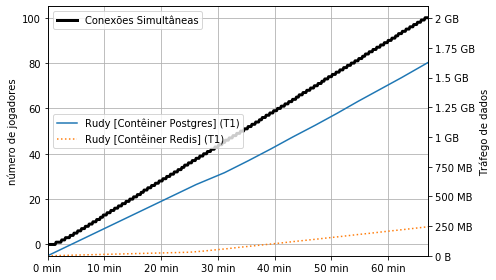
\includegraphics[width=.95\linewidth]{figuras/analise/rt/r_net_in_db.png}
        \caption{Bancos de Dados da arquitetura Rudy}
        \label{fig:r_netin_db}
    \end{subfigure}%
    \begin{subfigure}{0.5\textwidth}
        \centering
        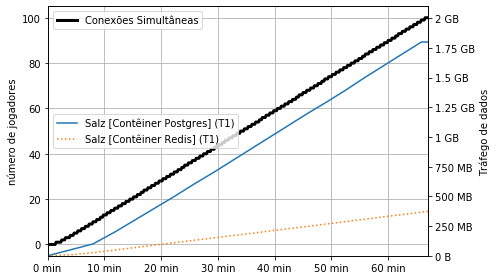
\includegraphics[width=.95\linewidth]{figuras/analise/rt/s_net_in_db.png}
        \caption{Bancos de Dados da arquitetura Salz}
        \label{fig:s_netin_db}
    \end{subfigure}\\

    \begin{subfigure}{0.5\textwidth}
        \centering
        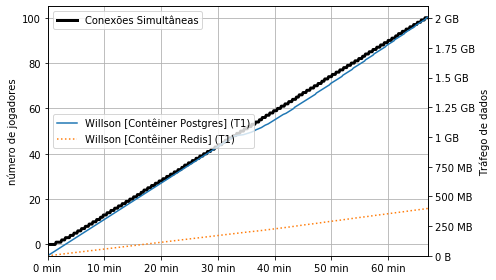
\includegraphics[width=.95\linewidth]{figuras/analise/rt/w_net_in_db.png}
        \caption{Bancos de Dados da arquitetura Willson}
        \label{fig:w_netin_db}
    \end{subfigure}

    Fonte: O próprio autor.
\end{figure}

A Figura~\ref{fig:experimento_db_net_in} exibe o comportamento da entrada dos dados para os bancos de dados.
%
Este segue um padrão visivelmente linear.
%
Ambas as arquiteturas consomem o banco de dados com o mesmo comportamento linear, entretanto em proporções diferentes.
%
Faz sentido analisar a vazão da rede do banco de dados.
%
Esta visualização está disponível na Figura~\ref{fig:net_in_db}.

\begin{figure}[htb!]
  \caption{Vazão da entrada de dados para a rede \textit{databases}.}
  \label{fig:net_in_db}
  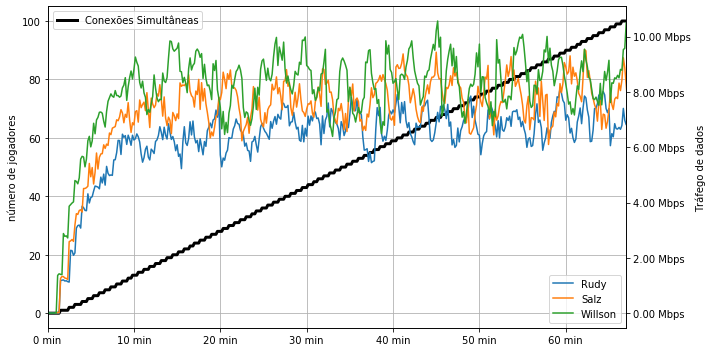
\includegraphics[width=0.8\textwidth]{figuras/analise/net_in_db.png}
  \centering

  Fonte: O próprio autor.
\end{figure}

A Figura~\ref{fig:net_in_db} exibe a existência de uma vazão máxima para entrada de dados aos bancos de dados.
%
Nota-se que existe diferença entre as arquiteturas, a qual já era visível na Figura~\ref{fig:experimento_db_net_in}.

Como existem pontos de contato entre as curvas, faz sentido realizar uma análise do comportamento médio.
%
A partir destes dados pode-se comparar as curvas e validar qual banco de dados recebeu mais requisições.
%
A Tabela~\ref{tab:net_in_db_media_quadrantes} exibe a média por quadrante das curvas comparado a vazão da rede por segundo.

\begin{table}[htb!]
\centering
\begin{adjustbox}{max width=\textwidth}
\caption{Consumo médio da entrada da rede por quadrante do PostgreSQL.}
\label{tab:net_in_db_media_quadrantes}

\begin{tabular}{l|l|l|l|l}
\hline \hline
Arquitetura & Primeiro Quadrante & Segundo Quadrante & Terceiro Quadrante & Quarto Quadrante \\ \hline \hline
Rudy        & 4,94 Mbps            & 6,67 Mbps           & 6,91 Mbps            & 7,03 Mbps          \\ \hline
Salz        & 6,06 Mbps            & 7,61 Mbps           & 7,88 Mbps            & 7,88 Mbps          \\ \hline
Willson     & 6,67 Mbps            & 8,34 Mbps          & 8,41 Mbps            & 8,55 Mbps          \\ \hline \hline
\end{tabular}
\end{adjustbox}

Fonte: O próprio autor.
\end{table}

A partir da Tabela~\ref{tab:net_in_db_media_quadrantes} percebe-se que a arquitetura Willson mesmo com características próximas a arquitetura Rudy, performou com melhor qualidade, recebendo mais dados de requisição.
%
O microsserviço \textit{rcrud} a qual poderia tornar-se um gargalo para a entrada de rede tem esta característica confirmada.

Ao comparar as arquiteturas Salz e Willson, percebe-se que, por mais que todos os seus microsserviços realizam conexão direta ao banco, existe uma diferença notória entre ambas as arquiteturas.
%
Esta diferença é dada pela quantidade de microsserviços na qual utilizam determinado banco de dados.

Nesse sentido, pode-se deduzir:

$$
    \overline{Entrada_{db\_r}} < \overline{Entrada_{db\_s}} < \overline{Entrada_{db\_w}}
$$

Deste modo, entende-se:

\begin{itemize}
 \item $\overline{Entrada_{db\_r}}$: Vazão de entrada média do banco de dados na arquitetura Rudy;
 \item $\overline{Entrada_{db\_r}}$: Vazão de entrada média do banco de dados na arquitetura Salz; e
 \item $\overline{Entrada_{db\_r}}$: Vazão de entrada média do banco de dados na arquitetura Willson.
\end{itemize}

A arquitetura Rudy contempla a menor vazão de rede entre as arquiteturas selecionadas.
%
A sua menor vazão, comparada as demais, é pelo afunilamento de requisições em um único microsserviço.
%
Dessa forma, o microsserviço \textit{rcrud} é um gargalo aparente nesta arquitetura.

A arquitetura Salz possui uma vazão de entrada maior comparado a arquitetura Rudy, porém menor que a arquitetura Willson.
%
Esta característica é dada pela saturação da \ac{cpu} do ponto de vista da arquitetura Salz, a qual obstruiu a vazão de dados.

A arquitetura Willson possui a maior vazão de entrada de dados entre as arquiteturas selecionadas.
%
Esta característica provém de um melhor aproveitamento da \ac{cpu} pela distribuição do processamento na arquitetura Willson.


\subsubsection{Microsserviços}

Considerando o ambiente de microsserviços, pode-se realizar a associação do número de jogadores simultâneos e entrada de rede consumida pelos contêineres de microsserviços.
%
Essa associação é realizada pelo tempo de registro das métricas.
%
O resultado desta associação pode ser visualizado na Figura~\ref{fig:experimento_gs_net_in}.

\begin{figure}[htb!]
    \caption{Entrada de dados da rede de microsserviços}
    \label{fig:experimento_gs_net_in}

    \begin{subfigure}{0.5\textwidth}
        \centering
        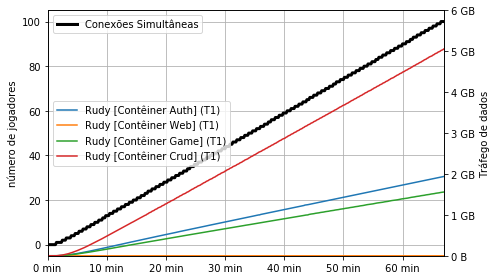
\includegraphics[width=.95\linewidth]{figuras/analise/rt/r_net_in_arch.png}
        \caption{Microsserviços da arquitetura Rudy}
        \label{fig:r_netin_gs}
    \end{subfigure}%
    \begin{subfigure}{0.5\textwidth}
        \centering
        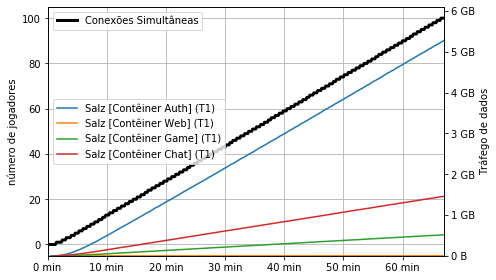
\includegraphics[width=.95\linewidth]{figuras/analise/rt/s_net_in_arch.png}
        \caption{Microsserviços da arquitetura Salz}
        \label{fig:s_netin_gs}
    \end{subfigure}\\

    \begin{subfigure}{0.5\textwidth}
        \centering
        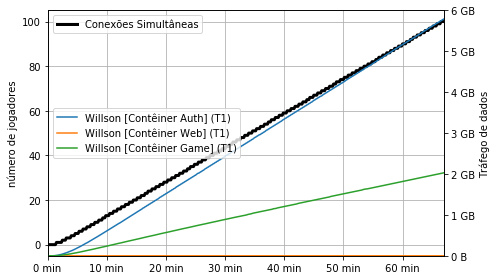
\includegraphics[width=.95\linewidth]{figuras/analise/rt/w_net_in_arch.png}
        \caption{Microsserviços da arquitetura Willson}
        \label{fig:w_netin_gs}
    \end{subfigure}

    Fonte: O próprio autor.
\end{figure}

A Figura~\ref{fig:experimento_gs_net_in} exibe o comportamento do consumo de entrada da rede, na qual visivelmente todos os serviços são lineares.
%
Dessa forma, pode-se deduzir os seguintes comportamentos para as arquiteturas de microsserviços:

$$
     Entrada_{rweb} < Entrada_{rgame} < Entrada_{rauth} < Entrada_{rcrud}
$$
$$
     Entrada_{sweb} < Entrada_{sgame} < Entrada_{schat} < Entrada_{sauth}
$$
$$
     Entrada_{wweb} < Entrada_{wgame} < Entrada_{wauth}
$$

Na qual entende-se:

\begin{itemize}
 \item $Entrada_{rweb}$: Curva de entrada do microsserviço \textit{web} na arquitetura Rudy;
 \item $Entrada_{rgame}$: Curva de entrada do microsserviço \textit{game} na arquitetura Rudy;
 \item $Entrada_{rauth}$: Curva de entrada do microsserviço \textit{auth} na arquitetura Rudy;
 \item $Entrada_{rcrud}$: Curva de entrada do microsserviço \textit{crud} na arquitetura Rudy;
  \item $Entrada_{sweb}$: Curva de entrada do microsserviço \textit{web} na arquitetura Salz;
 \item $Entrada_{sgame}$: Curva de entrada do microsserviço \textit{game} na arquitetura Salz;
 \item $Entrada_{sauth}$: Curva de entrada do microsserviço \textit{auth} na arquitetura Salz;
 \item $Entrada_{schat}$: Curva de entrada do microsserviço \textit{chat} na arquitetura Salz;
 \item $Entrada_{wweb}$: Curva de entrada do microsserviço \textit{web} na arquitetura Willson;
 \item $Entrada_{wgame}$: Curva de entrada do microsserviço \textit{game} na arquitetura Willson; e
 \item $Entrada_{wauth}$: Curva de entrada do microsserviço \textit{auth} na arquitetura Willson.
\end{itemize}


Este comportamento está diretamente relacionado a distribuição das funcionalidades dentro das arquiteturas.
%
A Subfigura~\ref{fig:r_netin_gs} exibe uma elevada carga de entrada consumida pelo microsserviço \textit{rcrud}, a qual está distribuída entre diversos processos nas demais arquiteturas.
%
Entretanto, para o microsserviço \textit{rcrud} ainda existe uma camada adicional de tráfego de dados para a realização da chamada ao microsserviço.

A partir do comportamento exibido nas Subfiguras~\ref{fig:r_netin_gs}, ~\ref{fig:s_netin_gs} e ~\ref{fig:w_netin_gs}, faz sentido analisar a vazão de rede de entrada.
%
Dessa forma pode-se analisar a limitação da entrada da rede.
%
O comportamento da vazão da rede de entrada de dados é visível na Figura~\ref{fig:net_in_gs}.

\begin{figure}[htb!]
  \caption{Vazão da entrada de dados para a rede \textit{gameservers}.}
  \label{fig:net_in_gs}
  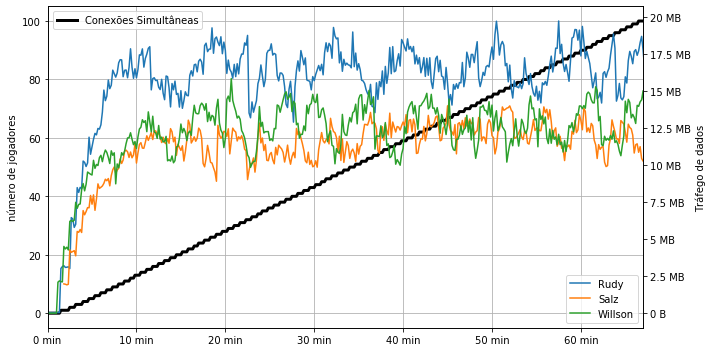
\includegraphics[width=0.8\textwidth]{figuras/analise/net_in_gs.png}
  \centering

  Fonte: O próprio autor.
\end{figure}

Conforme exibido na Figura~\ref{fig:net_in_gs}, a arquitetura Rudy contempla um maior consumo de entrada da rede.
%
Entretanto, as arquitetura Salz e Willson possuem, visualmente, o mesmo comportamento.
%
Dessa forma, faz sentido analisar a média dos quadrantes para quantificar e verificar se os valores médios são realmente próximos na arquitetura Salz e Willson.
%
A Tabela~\ref{tab:net_in_gs_media_quadrantes} exibe estes dados.

\begin{table}[htb!]
\centering
\begin{adjustbox}{max width=\textwidth}
\caption{Consumo médio da entrada da rede por quadrante do servidor de jogo.}
\label{tab:net_in_gs_media_quadrantes}

\begin{tabular}{l|l|l|l|l}
\hline \hline
Arquitetura & Primeiro Quadrante & Segundo Quadrante & Terceiro Quadrante & Quarto Quadrante \\ \hline \hline
Rudy        & 12,58 Mbps            & 15,62 Mbps           & 15,84 Mbps            & 15,66 Mbps          \\ \hline
Salz        & 9,22 Mbps            & 10,63 Mbps           & 11,97 Mbps            & 11,42 Mbps          \\ \hline
Willson     & 9,12 Mbps            & 12,30 Mbps          & 12,27 Mbps            & 12,23 Mbps          \\ \hline \hline
\end{tabular}
\end{adjustbox}

Fonte: O próprio autor.
\end{table}

A Tabela~\ref{tab:net_in_gs_media_quadrantes} exibe a média dos quadrantes da vazão de entrada dos servidores de jogo.
%
Dessa forma, podemos confirmar que a arquitetura Salz possui uma carga de entrada menor que a arquitetura Willson.
%
Entretanto, este aumento é um reflexo direto da comunicação interna da arquitetura ou do desempenho por uma otimização.

Nesse sentido, pode-se deduzir:

$$
    \overline{Entrada_{gs\_r}} < \overline{Entrada_{gs\_s}} < \overline{Entrada_{gs\_w}}
$$

Deste modo, entende-se:

\begin{itemize}
 \item $\overline{Entrada_{gs\_r}}$: Vazão de entrada médio dos microsserviços na arquitetura Rudy;
 \item $\overline{Entrada_{gs\_s}}$: Vazão de entrada médio dos microsserviços na arquitetura Salz; e
 \item $\overline{Entrada_{gs\_w}}$: Vazão de entrada médio dos microsserviços na arquitetura Willson.
\end{itemize}

A arquitetura Rudy possui um aumento excessivo em relação as demais arquiteturas selecionadas pela separação do microsserviço \textit{rcrud}.
%
Todas as chamadas, tanto ao Redis e PostgreSQL, passam por tal serviço.
%
Dessa forma, temos um aumento elevado em relação as demais arquiteturas.

A arquitetura Salz possui o menor valor de entrada.
%
Tal característica ocorre mesmo com a sincronização de posição de personagens entre os microsserviços \textit{sgame} e \textit{schat}.
%
Esta característica é resultante da comunicação direta com os microsserviços, a qual a arquitetura necessita de informações evitando reinjeção de dados na arquitetura de microsserviços.

A arquitetura Willson possui um valor intermediário em relação as demais arquiteturas selecionadas.
%
Este valor intermediário é dado pela vazão de requisições que a arquitetura Willson consegue exercer ao cliente.
%
Dessa forma, o tempo de resposta da arquitetura Willson  mostra-se menor que as demais, e consecutivamente elevando a frequência de requisições, a qual eleva a entrada do serviço como um todo.

\subsection{Saída de Rede}

Este experimento visa analisar o consumo da saída de rede unitariamente, em relação ao número de jogadores simultâneos.
%
Espera-se que o seu crescimento seja de tendência linear junto ao crescimento de jogadores concorrentes.
%
Neste contexto, existem os seguintes valores:

\begin{itemize}
    \item Jogadores simultâneos: Variável capturada a partir do microsserviço de jogo;
    \item Saída do serviço: Variável capturada a partir do monitor de recursos do Docker; e
    \item Saída do ambiente: Variável capturada a partir do sistema operacional.
\end{itemize}

Nota-se que o número de jogadores simultâneos e o consumo da saída de rede são indexados pelo tempo a qual tais dados foram capturados.
%
Nesse sentido, pode-se relacionar o número de jogadores simultâneos ao consumo de entrada de rede dos microsserviços e do banco de dados.
%
Dado tal contexto, faz sentido realizar uma análise separando os ambientes de Banco de Dados de Microsserviços.

\subsubsection{Banco de Dados}

Considerando o ambiente de banco de dados, pode-se realizar a associação de número de jogadores simultâneos e saída de rede consumida pelos contêineres de banco de dados.
%
Essa associação é realizada pelo tempo de registro das métricas.
%
O resultado desta associação pode ser visualizado na Figura~\ref{fig:experimento_db_net_out}.

\begin{figure}[htb!]
    \caption{Saída de dados da rede dos bancos de dados}
    \label{fig:experimento_db_net_out}

    \begin{subfigure}{0.5\textwidth}
        \centering
        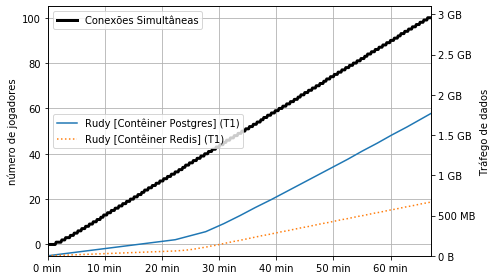
\includegraphics[width=.95\linewidth]{figuras/analise/rt/r_net_out_db.png}
        \caption{Bancos de Dados da arquitetura Rudy}
        \label{fig:r_netout_db}
    \end{subfigure}%
    \begin{subfigure}{0.5\textwidth}
        \centering
        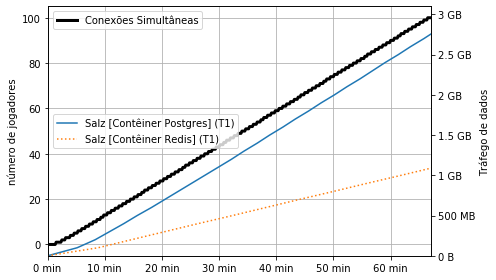
\includegraphics[width=.95\linewidth]{figuras/analise/rt/s_net_out_db.png}
        \caption{Bancos de Dados da arquitetura Salz}
        \label{fig:s_netout_db}
    \end{subfigure}\\

    \begin{subfigure}{0.5\textwidth}
        \centering
        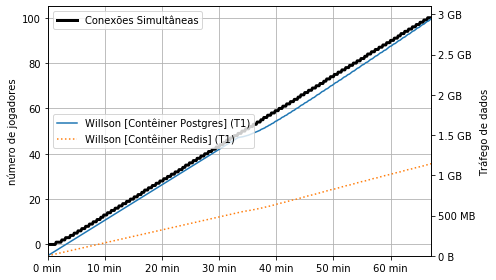
\includegraphics[width=.95\linewidth]{figuras/analise/rt/w_net_out_db.png}
        \caption{Bancos de Dados da arquitetura Willson}
        \label{fig:w_netout_db}
    \end{subfigure}

    Fonte: O próprio autor.
\end{figure}

Conforme visível na Figura~\ref{fig:experimento_db_net_out}, o comportamento da saída de dados corresponde diretamente a entrada de dados ao banco de dados.
%
Este comportamento era previsível, haja vista que o banco de dados recebe requisições as quais geram um determinada saída.
%
Faz sentido analisar a taxa de vazão total do ambiente de dados para fins comparativos a vazão de entrada.
%
O comportamento da vazão da rede de saída de dados é visível na Figura~\ref{fig:net_out_db}.

\begin{figure}[htb!]
  \caption{Vazão da saída de dados para a rede \textit{gameservers}.}
  \label{fig:net_out_db}
  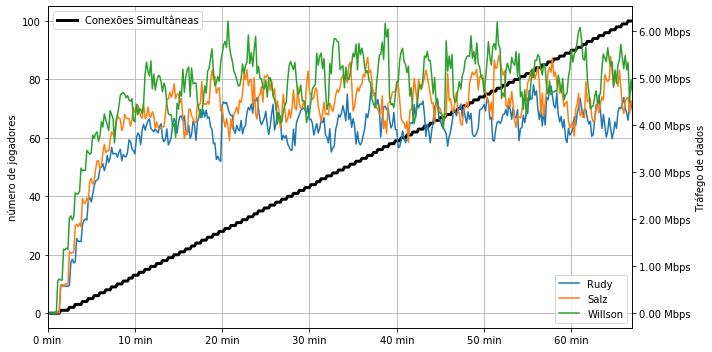
\includegraphics[width=0.8\textwidth]{figuras/analise/net_out_db.png}
  \centering

  Fonte: O próprio autor.
\end{figure}

Percebe-se que o comportamento de vazão de saída da rede segue o mesmo padrão da entrada de rede para a rede de banco de dados, tal característa é visível ao comparar a Figura~\ref{fig:net_out_db} e ~\ref{fig:net_in_db}.
%
Faz sentido analisar os quadrantes, validando se os valores encontrados de média de saída de rede seguem o comportamento da entrada de rede.
%
A Tabela~\ref{tab:net_out_db_media_quadrantes} exibe os valores de média de vazão de rede dos quadrantes.

\begin{table}[htb!]
\centering
\begin{adjustbox}{max width=\textwidth}
\caption{Consumo médio da saída da rede por quadrante do servidor de jogo.}
\label{tab:net_out_db_media_quadrantes}

\begin{tabular}{l|l|l|l|l}
\hline \hline
Arquitetura & Primeiro Quadrante & Segundo Quadrante & Terceiro Quadrante & Quarto Quadrante \\ \hline \hline
Rudy        & 2,93 Mbps            & 3,98 Mbps           & 4,10 Mbps            & 4,27 Mbps          \\ \hline
Salz        & 3,42 Mbps            & 4,57 Mbps           & 4,62 Mbps            & 4,63 Mbps          \\ \hline
Willson     & 3,65 Mbps            & 5,02 Mbps          & 5,10 Mbps            & 5,18 Mbps          \\ \hline \hline
\end{tabular}
\end{adjustbox}

Fonte: O próprio autor.
\end{table}

A partir da Tabela~\ref{tab:net_out_db_media_quadrantes}, percebe-se uma sequência para comparação entre as arquiteturas no critério referente a consumo de saída de rede.
%
Nesse sentido, pode-se deduzir:

$$
    \overline{Saida_{db\_r}} < \overline{Saida_{db\_s}} < \overline{Saida_{db\_w}}
$$

Deste modo, entende-se:

\begin{itemize}
 \item $\overline{Saida_{db\_r}}$: Vazão de saída média dos bancos de dados na arquitetura Rudy;
 \item $\overline{Saida_{db\_s}}$: Vazão de saída média dos bancos de dados na arquitetura Salz; e
 \item $\overline{Saida_{db\_w}}$: Vazão de saída média dos bancos de dados na arquitetura Willson.
\end{itemize}

O comportamento visual e a expressão deduzida a partir da média dos quadrantes entre arquiteturas extraídos é um reflexo direto da entrada de rede de banco de dados.
%
Dessa forma, podemos comparar a entrada e saída de rede, a fim de ter uma única comparação para vazão de rede sobre o ambiente de banco de dados.
%
Logo, pode-se comparar a expressão deduzida da Tabela~\ref{tab:net_out_db_media_quadrantes} com a expressão deduzida a partir da Tabela~\ref{tab:net_in_db_media_quadrantes} da seguinte forma:

$$
    \overline{Entrada_{db\_r}} < \overline{Entrada_{db\_s}} < \overline{Entrada_{db\_w}}
$$
$$
    \overline{Saida_{db\_r}} < \overline{Saida_{db\_s}} < \overline{Saida_{db\_w}}
$$

Deduz que:

$$
    \overline{Rede_{db\_r}} < \overline{Rede_{db\_s}} < \overline{Rede_{db\_w}}
$$

Na qual entende-se:

\begin{itemize}
 \item $\overline{Rede_{db\_r}}$: Vazão de rede média dos bancos de dados na arquitetura Rudy;
 \item $\overline{Rede_{db\_s}}$: Vazão de rede média dos bancos de dados na arquitetura Salz; e
 \item $\overline{Rede_{db\_w}}$: Vazão de rede média dos bancos de dados na arquitetura Willson.
\end{itemize}

\subsubsection{Microsserviços}

Considerando o ambiente de banco de dados, pode-se realizar a associação de número de jogadores simultâneos e saída de rede consumida pelos contêineres de banco de dados.
%
Essa associação é realizada pelo tempo de registro das métricas.
%
O resultado desta associação pode ser visualizado na Figura~\ref{fig:experimento_game_net_out}.

\begin{figure}[htb!]
    \caption{Saída de dados da rede dos microsserviços}
    \label{fig:experimento_game_net_out}

    \begin{subfigure}{0.5\textwidth}
        \centering
        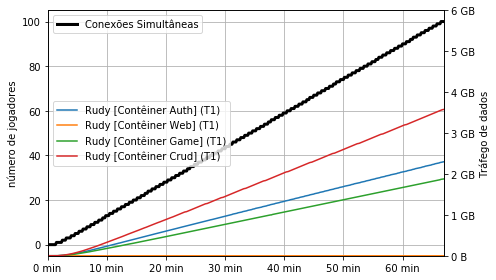
\includegraphics[width=.95\linewidth]{figuras/analise/rt/r_net_out_arch.png}
        \caption{Bancos de Dados da arquitetura Rudy}
        \label{fig:r_netout_arch}
    \end{subfigure}%
    \begin{subfigure}{0.5\textwidth}
        \centering
        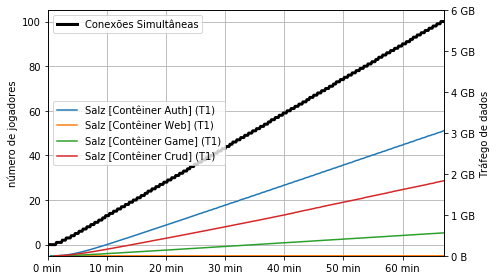
\includegraphics[width=.95\linewidth]{figuras/analise/rt/s_net_out_arch.png}
        \caption{Bancos de Dados da arquitetura Salz}
        \label{fig:s_netout_arch}
    \end{subfigure}\\

    \begin{subfigure}{0.5\textwidth}
        \centering
        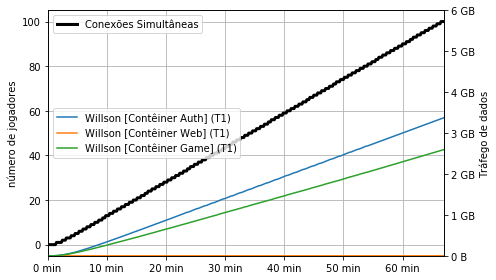
\includegraphics[width=.95\linewidth]{figuras/analise/rt/w_net_out_arch.png}
        \caption{Bancos de Dados da arquitetura Willson}
        \label{fig:w_netout_arch}
    \end{subfigure}

    Fonte: O próprio autor.
\end{figure}

A Figura~\ref{fig:experimento_game_net_out} exibe os mesmos comportamentos da entrada de rede.
%
A partir da Figura~\ref{fig:experimento_game_net_out}, pode-se deduzir os seguintes comportamentos para as arquiteturas de microsserviços:

$$
     Saida_{rweb} < Saida_{rgame} < Saida_{rauth} < Saida_{rcrud}
$$
$$
     Saida_{sweb} < Saida_{sgame} < Saida_{schat} < Saida_{sauth}
$$
$$
     Saida_{wweb} < Saida_{wgame} < Saida_{wauth}
$$

Na qual entende-se:

\begin{itemize}
 \item $Saida_{rweb}$: Curva de saída do microsserviço web na arquitetura Rudy;
 \item $Saida_{rgame}$: Curva de saída do microsserviço game na arquitetura Rudy;
 \item $Saida_{rauth}$: Curva de saída do microsserviço auth na arquitetura Rudy;
 \item $Saida_{rcrud}$: Curva de saída do microsserviço crud na arquitetura Rudy;
  \item $Saida_{sweb}$: Curva de saída do microsserviço web na arquitetura Salz;
 \item $Saida_{sgame}$: Curva de saída do microsserviço game na arquitetura Salz;
 \item $Saida_{sauth}$: Curva de saída do microsserviço auth na arquitetura Salz;
 \item $Saida_{schat}$: Curva de saída do microsserviço chat na arquitetura Salz;
 \item $Saida_{wweb}$: Curva de saída do microsserviço web na arquitetura Willson;
 \item $Saida_{wgame}$: Curva de saída do microsserviço game na arquitetura Willson; e
 \item $Saida_{wauth}$: Curva de saída do microsserviço auth na arquitetura Willson.
\end{itemize}

A partir da dedução da Figura~\ref{fig:experimento_game_net_out}, pode-se dizer que o comportamento de entrada e saída dos microsserviços seguem a mesma tendência.
%
Nesse sentido, pode-se apresentar a seguinte dedução:

$$
     Rede_{rweb} < Rede_{rgame} < Rede_{rauth} < Rede_{rcrud}
$$
$$
     Rede_{sweb} < Rede_{sgame} < Rede_{schat} < Rede_{sauth}
$$
$$
     Rede_{wweb} < Rede_{wgame} < Rede_{wauth}
$$

Na qual entende-se:

\begin{itemize}
 \item $Rede_{rweb}$: Consumo da rede do microsserviço web na arquitetura Rudy;
 \item $Rede_{rgame}$: Consumo da rede do microsserviço game na arquitetura Rudy;
 \item $Rede_{rauth}$: Consumo da rede do microsserviço auth na arquitetura Rudy;
 \item $Rede_{rcrud}$: Consumo da rede do microsserviço crud na arquitetura Rudy;
  \item $Rede_{sweb}$: Consumo da rede do microsserviço web na arquitetura Salz;
 \item $Rede_{sgame}$: Consumo da rede do microsserviço game na arquitetura Salz;
 \item $Rede_{sauth}$: Consumo da rede do microsserviço auth na arquitetura Salz;
 \item $Rede_{schat}$: Consumo da rede do microsserviço chat na arquitetura Salz;
 \item $Rede_{wweb}$: Consumo da rede do microsserviço web na arquitetura Willson;
 \item $Rede_{wgame}$: Consumo da rede do microsserviço game na arquitetura Willson; e
 \item $Rede_{wauth}$: Consumo da rede do microsserviço auth na arquitetura Willson.
\end{itemize}

Além da análise do comportamento de consumo de rede, a partir da saída da rede faz sentido analisar a vazão da rede por todos os microsserviços operando juntos.
%
A Figura~\ref{fig:net_in_gs} exibe a vazão de rede ao longo do tempo do experimento.

\begin{figure}[htb!]
  \caption{Vazão da saída de dados para a rede \textit{gameservers}.}
  \label{fig:net_in_gs}
  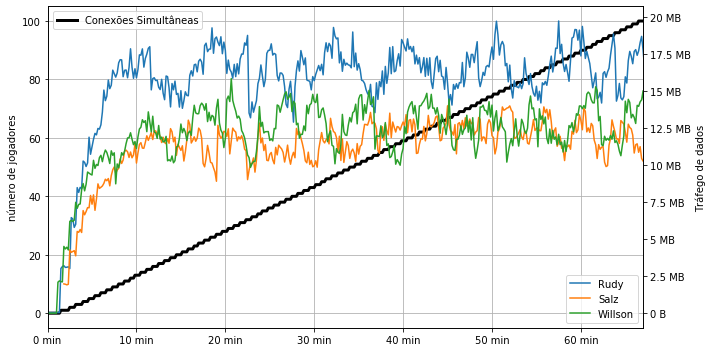
\includegraphics[width=0.8\textwidth]{figuras/analise/net_in_gs.png}
  \centering

  Fonte: O próprio autor.
\end{figure}

A partir da Figura~\ref{fig:net_in_gs}, percebe-se um maior consumo pela arquitetura Rudy.
%
Este comportamento era previsível pela relação com a rede de entrada.
%
Entretanto, as arquiteturas Salz e Willson não seguem o mesmo comportamento.
%
Dessa forma, faz sentido realizar uma análise por quadrantes a partir da vazão de dados.
%
Estes dados são visíveis na Figura~\ref{tab:net_out_gs_media_quadrantes}.

\begin{table}[htb!]
\centering
\begin{adjustbox}{max width=\textwidth}
\caption{Consumo médio da saída da rede por quadrante do servidor de jogo.}
\label{tab:net_out_gs_media_quadrantes}

\begin{tabular}{l|l|l|l|l}
\hline \hline
Arquitetura & Primeiro Quadrante & Segundo Quadrante & Terceiro Quadrante & Quarto Quadrante \\ \hline \hline
Rudy        & 13,91 Mbps            & 17,50 Mbps           & 17,08 Mbps            & 17,41 Mbps          \\ \hline
Salz        & 12,34 Mbps            & 15,01 Mbps           & 13,85 Mbps            & 14,84 Mbps          \\ \hline
Willson     & 12,93 Mbps            & 15,46 Mbps          & 15,39 Mbps            & 15,66 Mbps          \\ \hline \hline
\end{tabular}
\end{adjustbox}

Fonte: O próprio autor.
\end{table}

A partir dos valores obtidos na Tabela~\ref{tab:net_out_gs_media_quadrantes} pode-se deduzir a relação de consumo de rede.
%
A partir da Tabela~\ref{tab:net_in_db_media_quadrantes}, percebe-se uma sequência para comparação entre as arquiteturas no critério referente a consumo de saída de rede.
%
Nesse sentido, pode-se deduzir:

$$
    \overline{Saida_{gs\_s}} < \overline{Saida_{gs\_w}} < \overline{Saida_{gs\_r}}
$$

Deste modo, entende-se:

\begin{itemize}
 \item $\overline{Saida_{gs\_r}}$: Vazão de saída média dos microsserviços na arquitetura Rudy;
 \item $\overline{Saida_{gs\_s}}$: Vazão de saída média dos microsserviços na arquitetura Salz; e
 \item $\overline{Saida_{gs\_w}}$: Vazão de saída média dos microsserviços na arquitetura Willson.
\end{itemize}

\section{Análise unificada dos resultados}
\label{sec:experimentos_conc}

Este capítulo descreve os resultados obtidos a partir dos experimentos executados sobre as arquiteturas Rudy, Salz e Willson.
%
Tais experimentos foram baseados em um protocolo de execução, a qual garante a limpeza do ambiente evitando interferência de demais execuções.

Foram obtidas comparações ao realizar uma análise individual dos critérios obtidos nos experimentos.
%
É possível realizar um aglomerado de todos os resultados em uma única tabela.
%
A Tabela~\ref{tab:resultados_experimentos} exibe as comparações obtidas a partir dos dados capturados.

\begin{table}[htb!]
\centering
\begin{adjustbox}{max width=\textwidth}
\caption{Resultados obtidos a partir dos dados capturados.}
\label{tab:resultados_experimentos}

\begin{tabular}{l|l||l|l|l}
\hline \hline
\multicolumn{2}{l||}{Critério}                                                                          & Rudy        & Salz        & Willson     \\ \hline \hline
\multirow{7}{*}{\begin{tabular}[c]{@{}l@{}}Tempo\\ de Resposta\end{tabular}}  & Criar Conta           & Maior valor & Valor médio & Menor valor \\ \cline{2-5} 
                                                                                & Criar Personagem      & Maior valor & Valor médio & Menor valor \\ \cline{2-5} 
                                                                                & Iniciar Sessão        & Maior valor & Menor valor & Valor médio \\ \cline{2-5} 
                                                                                & Instanciar Personagem & Valor médio & Maior valor & Menor valor \\ \cline{2-5} 
                                                                                & Movimentar Personagem & Valor médio & Maior valor & Menor valor \\ \cline{2-5} 
                                                                                & Enviar Mensagem       & Maior valor & Valor médio & Menor valor \\ \cline{2-5} 
                                                                                & Receber Mensagem      & Maior valor & Valor médio & Menor valor \\ \hline \hline
\multirow{2}{*}{\begin{tabular}[c]{@{}l@{}}Consumo\\ de CPU\end{tabular}}     & Banco de Dados        & Menor valor & Valor médio & Maior valor \\ \cline{2-5} 
                                                                                & Microsserviços        & Valor médio & Menor valor & Maior valor \\ \hline \hline
\multirow{2}{*}{\begin{tabular}[c]{@{}l@{}}Consumo\\ de Memória\end{tabular}} & Banco de Dados        & Menor valor & Valor médio & Maior valor \\ \cline{2-5} 
                                                                                & Microsserviços        & Valor médio & Maior valor & Menor valor \\ \hline \hline
\multirow{2}{*}{\begin{tabular}[c]{@{}l@{}}Entrada\\ de Rede\end{tabular}}    & Banco de Dados        & Menor valor & Valor médio & Maior valor \\ \cline{2-5} 
                                                                                & Microsserviços        & Menor valor & Valor médio & Maior valor \\ \hline \hline
\multirow{2}{*}{\begin{tabular}[c]{@{}l@{}}Saída\\ de Rede\end{tabular}}      & Banco de Dados        & Menor valor & Valor médio & Maior valor \\ \cline{2-5} 
                                                                                & Microsserviços        & Maior valor & Valor médio & Menor valor \\ \hline \hline
\end{tabular}
\end{adjustbox}

Fonte: O próprio autor.
\end{table}

A partir da Tabela~\ref{tab:resultados_experimentos}, podemos observar comportamentos aproximados, na qual respeitam as relações obtidas.
%
Faz sentido simplificar os resultados obtidos, exibidos na Tabela~\ref{tab:resultados_experimentos}, justificando pelo funcionamento das arquiteturas.
%
A seguir, listamos as deduções obtidas:

\begin{itemize}
 \item \textbf{Criar Conta} e \textbf{Criar Personagem} são operações que utilizam o mesmo fluxo e protocolo para persistência de dados no mesmo banco de dados. Ambos possuem o mesmo comportamento;
 \item \textbf{Instanciar Personagem} e \textbf{Movimentar Personagem} são ações que utilizam o mesmo fluxo e protocolo. Ambos possuem o mesmo comportamento;
 \item \textbf{Enviar Mensagem} e \textbf{Receber Mensagem} são ações que utilizam o mesmo fluxo e protocolo. Ambos possuem o mesmo comportamento; e
 \item \textbf{Entrada de Rede} do banco de dados e do microsserviços cresce proporcionalmente.
\end{itemize}

A partir destas deduções, é possível simplificar a Tabela~\ref{tab:resultados_experimentos}.
%
A Tabela~\ref{tab:resultados_experimentos_simplificados} exibe os comportamentos obtidos de forma simplificada.


\begin{table}[htb!]
\centering
\begin{adjustbox}{max width=\textwidth}
\caption{Resultados obtidos a partir dos dados capturados.}
\label{tab:resultados_experimentos_simplificados}

\begin{tabular}{l|l||l|l|l}
\hline \hline
\multicolumn{2}{l||}{Critério}                                                                     & Rudy        & Salz        & Willson     \\ \hline \hline
\multirow{4}{*}{\begin{tabular}[c]{@{}l@{}}Tempo\\ de Resposta\end{tabular}}  & Operações Web      & Maior valor & Valor médio & Menor valor \\ \cline{2-5}
                                                                              & Operação de Sessão & Maior valor & Menor valor & Valor médio \\ \cline{2-5} 
                                                                              & Operações do Mundo & Valor médio & Maior valor & Menor valor \\ \cline{2-5} 
                                                                              & Operações de Chat  & Maior valor & Valor médio & Menor valor \\ \hline \hline
\multirow{2}{*}{\begin{tabular}[c]{@{}l@{}}Consumo\\ de CPU\end{tabular}}     & Banco de Dados     & Menor valor & Valor médio & Maior valor \\ \cline{2-5} 
                                                                              & Microsserviços     & Valor médio & Menor valor & Maior valor \\ \hline \hline
\multirow{2}{*}{\begin{tabular}[c]{@{}l@{}}Consumo\\ de Memória\end{tabular}} & Banco de Dados     & Menor valor & Valor médio & Maior valor \\ \cline{2-5} 
                                                                              & Microsserviços     & Valor médio & Maior valor & Menor valor \\ \hline \hline
\multicolumn{2}{l||}{Entrada de Rede}                                                              & Menor valor & Valor médio & Maior valor \\ \hline \hline
\multirow{2}{*}{\begin{tabular}[c]{@{}l@{}}Saída\\ de Rede\end{tabular}}      & Banco de Dados     & Menor valor & Valor médio & Maior valor \\ \cline{2-5} 
                                                                              & Microsserviços     & Maior valor & Valor médio & Menor valor \\ \hline \hline
\end{tabular}
\end{adjustbox}

Fonte: O próprio autor.
\end{table}

A Tabela~\ref{tab:resultados_experimentos_simplificados} exibe a tabela simplificada.
%
A partir destes dados, conclui-se que:

\begin{itemize}
 \item \textbf{Operação de Sessão} é uma categoria de requisições que não compartilha características com outras operações;
 \item \textbf{Consumo de CPU do Banco de Dados} é inversamente proporcional a requisições web \textbf{Criar Conta} e \textbf{Criar Personagem};
 \item \textbf{Consumo de CPU dos microsserviços} é inversamente proporcional a maioria das ações que envolvem o serviço de jogo sobre o protocolo \ac{rpc};
 \item \textbf{Saída de Rede dos bancos de dados} relaciona-se a entrada de rede do banco de dados, que consecutivamente tem relação com \textbf{Operações Web}; e
 \item \textbf{Saída de Rede dos microsserviços} relaciona-se  as requisições da operação de mundo, visto que tais operações possuem alta frequência de requisições.
\end{itemize}

\section{Considerações parciais}

Este capítulo teve como objetivo descrever os resultados obtidos, a partir da execução dos experimentos sobre as arquiteturas de microsserviços Rudy, Salz e Willson.
%
Dessa forma, tal capítulo exibe os seguintes experimentos:

\begin{itemize}
 \item Tempo de resposta;
 \item Consumo de \ac{cpu};
 \item Consumo de Memória;
 \item Entrada de Rede; e
 \item Saída de Rede;
\end{itemize}

A partir do tempo de resposta, pode-se observar quatro comportamentos distintos.
%
Os comportamentos observados são:

\begin{itemize}
 \item Operações Web: A arquitetura Willson mostrou o menor tempo de resposta justificado por uma melhor ocupação de \ac{cpu} e conexão direta ao banco de dados;
 \item Operação de Sessão: A arquitetura Salz mostrou o menor tempo de resposta justificado por fornecer o microsserviço de autenticação de forma pública para conexão pelo cliente, diminuindo a cadeia de conexões necessárias para realizar a autenticação no serviço;
 \item Operações de Mundo: A arquitetura Willson mostrou o menor tempo de resposta justificado por um melhor aproveitamento de \ac{cpu};
 \item Operações do Mundo: A arquitetura Willson mostrou o menor tempo de resposta justificado por um melhor aproveitamento de \ac{cpu}; e
 \item Operações de Chat: A arquitetura Willson mostrou o menor tempo de resposta justificado por um melhor aproveitamento de \ac{cpu};
\end{itemize}

A partir dos resultados obtidos, pode-se avaliar a arquitetura Willson como a melhor arquitetura para o critério de tempo de resposta.
%
Entretanto, para obter determinado desempenho, o seu consumo de recursos é maior, no geral, que as demais arquiteturas.


A partir dos resultados de consumo de \ac{cpu}, foi dividido o ambiente em banco de dados e microsserviços.
%
Para a arquitetura do banco de dados, a arquitetura Rudy obteve o menor consumo de \ac{cpu} em média.
%
Tal resultado é proveniente do enfileiramento de requisições pelo microsserviço \textit{rcrud}, a qual obstrui a comunicação com o banco de dados, tornando uma comunicação serial.

Para a arquitetura de microsserviços, a arquitetura Salz obteve o menor consumo de \ac{cpu} em média.
%
Este resultado é proveniente da divisão dos microsserviços \textit{sgame} e \textit{schat}, na qual obstruem a \ac{cpu} com comunicação interna.

Para o critério de consumo de memória na infraestrutura do banco de dados, a arquitetura Rudy toma a posição como mais econômica, na qual mostra um ponto positivo para a obstrução das requisições no microsserviço \textit{rcrud}.
%
Isto é um reflexo positivo direto da minimização de requisições simultâneas a um serviço de fonte de dados.


Para o consumo de memória por parte do serviço a arquitetura Willson mostrou-se a mais econômica.
%
Esta economia de memória é proveniente da minimização da quantidade de microsserviços, e consecutivamente de processos concorrentes para execução das mesmas tarefas.
%
Entretanto, este ponto não necessariamente é positivo, mas sim uma característica do experimento.
Nota-se que no caso da necessidade de escalar a arquitetura Willson será obrigatório escalar sistemas que talvez sejam desnecessários para a operação do serviço.

Para o tráfego de rede, notou-se que a entrada e saída de dados no banco de dados tendem a crescer com a mesma intensidade.
%
Esta característica é dada pelo protocolo utilizado ao consumir um dado do banco de dados, na qual sempre haverá uma resposta sobre a requisição enviada.
%
Dentro deste contexto, a arquitetura Rudy mostrou utilizar menos banco de dados.
%
Isto é um reflexo direto ao enfileiramento causado pelo microsserviço \textit{rcrud}.

Entretanto, isolando o ambiente de microsserviços no critério de saída de rede, possui o menor e maior consumo para os ambientes de banco de dados e microsserviços respectivamente.
%
Esta característica é dada pelo elevado consumo de rede interna para realizar consultas ao banco de dados, devido ao microsserviço \textit{rcrud}.

